% ---
% Modelo de Tese/Dissertação
% Autora: Fabiana Frata Furlan Peres 
% 2014 
% ---
% ADAPTADO DE:
% modelo de Documento TCC da Unioeste   
%
% que por sua vez foi ADAPTADO DE: 
% abtex2-modelo-trabalho-academico.tex, v-1.6 laurocesar
% Copyright 2012-2013 by abnTeX2 group at http://abntex2.googlecode.com/ 
% ---
% abnTeX2: Modelo de Trabalho Academico (tese de doutorado, dissertacao de
% mestrado e trabalhos monograficos em geral) em conformidade com 
% ABNT NBR 14724:2011: Informacao e documentacao - Trabalhos academicos - Apresentacao
%
% ---
% DECLARAÇÃO DO TIPO DE DOCUMENTO, TAMANHO DA FOLHA E FONTE
% ---
\documentclass[12pt,oneside,a4paper,english,french,spanish,listof=entryprefix]{abntex2}

% ---
% DEFINIÇÃO DOS PACOTES UTILIZADOS
% ---
\usepackage{cmap}				% Mapear caracteres especiais no PDF
\usepackage{lmodern}			% Usa a fonte Latin Modern			
\usepackage[T1]{fontenc}			% Selecao de codigos de fonte.
\usepackage[utf8]{inputenc}		% Codificacao do documento (conversão automática dos acentos)
\usepackage{lastpage}			% Usado pela Ficha catalográfica
\usepackage{indentfirst}			% Indenta o primeiro parágrafo de cada seção.
\usepackage{color}				% Controle das cores
\usepackage{graphicx}			% Inclusão de gráficos

\usepackage{lipsum}			

\usepackage{amsmath}
\usepackage{amssymb}

% ---
% CONFIGURAÇÕES PARA CÓDIGO FONTE
% ---
\usepackage{listings}
\usepackage{scrhack}
\usepackage{chngcntr}
 
\definecolor{codegreen}{rgb}{0,0.6,0}
\definecolor{codegray}{rgb}{0.5,0.5,0.5}
\definecolor{whitesmoke}{rgb}{0.96, 0.96, 0.96}
\definecolor{deepcarminepink}{rgb}{0.94, 0.19, 0.22}
\definecolor{tearose(orange)}{rgb}{0.97, 0.51, 0.47}
\definecolor{tealgreen}{rgb}{0.0, 0.51, 0.5}
\definecolor{teagreen}{rgb}{0.82, 0.94, 0.75}
\definecolor{tealblue}{rgb}{0.21, 0.46, 0.53}
 
\lstdefinestyle{mystyle}{
    backgroundcolor=\color{whitesmoke},   
    commentstyle=\color{codegreen},
    keywordstyle=\color{deepcarminepink},
    numberstyle=\tiny\color{tealblue},
    stringstyle=\color{tealgreen},
    basicstyle=\footnotesize,
    breakatwhitespace=false,         
    breaklines=true,        
    prebreak=\raisebox{0ex}[0ex][0ex]{\ensuremath{\hookleftarrow}},         
    captionpos=b,                    
    keepspaces=true,                 
    numbers=left,                    
    numbersep=5pt,                  
    showspaces=false,                
    showstringspaces=false,
    showtabs=false,                  
    tabsize=2
}
 
\lstset{style=mystyle}
\renewcommand{\lstlistingname}{Código}

% Fonte "Arial"
% ---
\usepackage{helvet}
\renewcommand{\familydefault}{\sfdefault}

% Pacotes de citações
% ---
\usepackage[alf,abnt-emphasize=bf,bibjustif]{abntex2cite}

% ---
% CONFIGURAÇÕES DA APARENCIA DO PDF FINAL
% ---
\definecolor{blue}{RGB}{41,5,195}	% alterando o aspecto da cor azul
\makeatletter
\hypersetup{     	
		pdftitle={\@title}, 
		pdfauthor={\@author},
    	pdfsubject={\imprimirpreambulo},
	    pdfcreator={LaTeX with abnTeX2},
		pdfkeywords={abnt}{latex}{abntex}{abntex2}{trabalho acadêmico}, 
		colorlinks=true,       		% false: boxed links; true: colored links
    	linkcolor=black,          	% color of internal links
    	citecolor=black,        		% color of links to bibliography
    	filecolor=magenta,      		% color of file links
		urlcolor=blue,
		bookmarksdepth=4
}
\makeatother

% ---
% INFORMAÇÕES REFERENTE A DISSERTAÇÃO
% ---
\titulo{TCC sobre Java}
\autor{Jorge Silva \\ Silva Matheus}
\orientador{Msc. Nome do Orientador}
\coorientador{Prof. Esp. Nome do Coorientador}
\data{2016}
 % DADOS para CAPA e FOLHA DE ROSTO

% ---
% CAPA
% ---
\renewcommand{\imprimircapa}{%
  \begin{capa}
  	\begin{center}
  		\large{FACULDADE ANGLO-AMERICANO DE FOZ DO IGUAÇU}
  	\end{center}
    \center
    %{\imprimirautor}
        
    %{\ABNTEXchapterfont\large\imprimirautor} % Original
    {\ABNTEXchapterfont\imprimirautor}

    \vspace*{8cm}
    %{\imprimirtitulo}
    \ABNTEXchapterfont\bfseries\large\imprimirtitulo
    \vfill
    
    \imprimirlocal

    \imprimirdata
    
    \vspace*{1cm}
  \end{capa}
}

\makeatletter
% ---
% FOLHA DE ROSTO
% ---
\renewcommand{\folhaderostocontent}{
		\center	
		%{\large\textbf\imprimirautor} %Original
			{\large\imprimirautor}
	
	    \vspace*{8cm}		
		
		
		{\large\textbf\imprimirtitulo}
	
		\vspace*{3cm}	

		\abntex@ifnotempty{\imprimirpreambulo}{
			\hspace{.3\textwidth}
			\begin{minipage}{.55\textwidth}
			
				\SingleSpacing
				\imprimirpreambulo				
				\SingleSpacing				
				{\imprimirorientadorRotulo~\imprimirorientador\par}
				\SingleSpacing	
		        \abntex@ifnotempty{\imprimircoorientador}{
		             {\imprimircoorientadorRotulo~\imprimircoorientador}
		}
		\end{minipage}
		
			\vspace*{\fill}
		}
		
		
		{\large\textbf\imprimirlocal}
		
		{\large\textbf\imprimirdata}		
}

% ---
% OUTRAS CONFIGURAÇÕES
% ---
\setlength{\parindent}{1.3cm} 		% Tamanho do parágrafo
\setlength{\parskip}{0.2cm}  		% Controle do espaçamento entre um parágrafo e outro
	
% Altera o tamanho das fontes dos capítulos e dos apêndices
% ---
\renewcommand{\ABNTEXchapterfont}{\bfseries}
\renewcommand{\ABNTEXchapterfontsize}{\large}
\renewcommand{\ABNTEXsectionfontsize}{\normalfont}

% ---
% SEPARAÇÃO DE PALAVRAS
% ---
%\hyphenation{}
\hyphenation{teorias}
\hyphenation{baseados}
\hyphenation{MATLAB}
\hyphenation{Pyramid}
\hyphenation{Mar-cação}
\hyphenation{lin-guagem}
\hyphenation{matplotlib}
\hyphenation{sociali-zação}
\hyphenation{bi-bli-oteca}
\hyphenation{Notebook}
\hyphenation{profis-si-onais}
\hyphenation{ar-quivos}
\hyphenation{usu-ário}
\hyphenation{fer-ramentas}
\hyphenation{materi-al}
\hyphenation{re-almen-te}
\hyphenation{LinkedIn}
\hyphenation{proces-samento}
\hyphenation{neces-sidades}

% Configura layout para elementos textuais
% -
\makepagestyle{abnt_ufpr}

\makeoddhead{abntchapfirst}{}{}{\ABNTEXfontereduzida\thepage}

\pagestyle{abnt_ufpr}

\newtheorem{theorem}{Teorema}[chapter]
\newtheorem{definition}[theorem]{Defini\c{c}\~{a}o}
\newtheorem{proposition}[theorem]{Proposi\c{c}\~{a}o}

\makeatother

% ---
% CONFIGURAÇÃO DE LISTAS DE CONTEÚDO
% ---
% lista de gráficos
% -
\newcommand{\graficoname}{GRÁFICO}
\newcommand{\listofgraficosname}{LISTA DE GRÁFICOS}

\newfloat[chapter]{grafico}{loq}{\graficoname}
\newlistof{listofgraficos}{loq}{\listofgraficosname}
\newlistentry{grafico}{loq}{0}

\counterwithout{grafico}{chapter}		% configurações para atender às regras da ABNT em listas
\renewcommand{\cftgraficoname}{\graficoname\space}
\renewcommand*{\cftgraficoaftersnum}{\hfill--\hfill}

% lista de códigos
% -
\renewcommand{\lstlistingname}{CÓDIGO}
\renewcommand{\lstlistlistingname}{LISTA DE CÓDIGOS}

\begingroup\makeatletter				% configurações para atender às regras da ABNT em listas
\let\newcounter\@gobble\let\setcounter\@gobbletwo
  \globaldefs\@ne \let\c@loldepth\@ne
  \newlistof{listings}{lol}{\lstlistlistingname}
  \newlistentry{lstlisting}{lol}{0}
\endgroup

\renewcommand{\cftlstlistingaftersnum}{\hfill--\hfill}

\let\oldlstlistoflistings\lstlistoflistings
\renewcommand{\lstlistoflistings}{%
   \begingroup%
   \let\oldnumberline\numberline%
   \renewcommand{\numberline}{\lstlistingname\space\oldnumberline}%
   \oldlstlistoflistings%
   \endgroup}

%\setlength{\parindent}{1.3cm} 			% Tamanho do parágrafo
%\setlength{\parskip}{0.0cm}  			% Controle do espaçamento entre um parágrafo e outro

% Altera o tamanho das fontes dos capítulos e dos apêndices
% -
\renewcommand{\ABNTEXchapterfont}{\normalfont\fontseries{b}\selectfont}
\renewcommand{\ABNTEXchapterfontsize}{\normalsize}
\renewcommand{\ABNTEXpartfont}{\fontseries{b}\selectfont\selectfont}
\renewcommand{\ABNTEXpartfontsize}{\normalsize}
\renewcommand{\ABNTEXsectionfont}{\normalfont\selectfont}
\renewcommand{\ABNTEXsectionfontsize}{\normalsize}
\renewcommand{\ABNTEXsubsectionfont}{\normalfont\selectfont}
\renewcommand{\ABNTEXsubsectionfontsize}{\normalsize}
\renewcommand{\ABNTEXsubsubsectionfont}{\normalfont\selectfont}
\renewcommand{\ABNTEXsubsubsectionfontsize}{\normalsize}
\renewcommand{\ABNTEXsubsubsubsectionfont}{\normalfont\itshape\selectfont}
\renewcommand{\ABNTEXsubsubsubsectionfontsize}{\normalsize}

% ---
% CONFIGURAÇÃO DO SUMÁRIO
% ---
% Sumário
\renewcommand*{\cftsectionfont}{\normalfont}
\renewcommand*{\cftsubsubsectionfont}{\normalfont}
\renewcommand*{\cftsubsectionfont}{\normalfont}
\renewcommand*{\cftparagraphfont}{\normalfont\itshape}

% ---
% Modifica o espaçamento no sumário
% Nao ha espacos, para as entradas de capitulos
% ---
\setlength{\cftbeforeparagraphskip}{0pt}
\setlength{\cftbeforesubsectionskip}{0pt}
\setlength{\cftbeforesectionskip}{0pt}
\setlength{\cftbeforesubsubsectionskip}{0pt}
\setlength{\cftbeforechapterskip}{0pt}

% ---
% CAPITALIZAÇÃO DE LISTAS
% ---

\addto\captionsbrazil{
	\renewcommand{\bibname}{REFER\^ENCIAS}
}
\addto\captionsbrazil{\renewcommand{\listadesiglasname}{LISTA DE ABREVIATURAS}}
\addto\captionsbrazil{\renewcommand{\listfigurename}{LISTA DE ILUSTRAÇÕES}}
\addto\captionsbrazil{\renewcommand{\listtablename}{LISTA DE TABELAS}}
%\addto\captionsbrazil{%
%  \renewcommand*{\lstlistlistingname}{LISTA DE CÓDIGOS}%
%  \renewcommand*{\lstlistingname}{CÓDIGO}%
%}
\addto\captionsbrazil{\renewcommand{\contentsname}{SUMÁRIO}}
\addto\captionsbrazil{\renewcommand\appendixtocname{APÊNDICES}\renewcommand\appendixpagename{APÊNDICES}}
\addto\captionsbrazil{\renewcommand{\figurename}{FIGURA}}
\addto\captionsbrazil{\renewcommand{\tablename}{TABELA}}

% ---
% LAYOUT PARA ELEMENTOS TEXTUAIS
% ---
%\makepagestyle{abnt_ufpr}

%\makeoddhead{abntchapfirst}{}{}{\ABNTEXfontereduzida\thepage}

%\pagestyle{abnt_ufpr}

% ---
% AMBIENTES
% ---
%\newtheorem{teo}{Teorema}[chapter]
%\newtheorem{cor}[teo]{Corol\'{a}rio}
%\newtheorem{lem}[teo]{Lema}
%\newtheorem{prop}[teo]{Proposi\c{c}\~{a}o}
%\newtheorem{defn}[teo]{Defini\c{c}\~{a}o}
%\newtheorem{Ex}[teo]{Exemplo}
%\newtheorem{obs}[teo]{Observa\c{c}\~{a}o}
%\newtheorem{prob}[teo]{Problema}
%\newtheorem{conc}[teo]{Conclusão}
%\newenvironment{dem}{\smallskip \noindent{\bf Demonstra\c{c}\~{a}o}: }
%{\hfill $\Box$\hspace{0in}\medskip}

% ---
% COMANDOS FREQUENTES
% ---
%\newcommand{\eq}{\begin{equation}}
%	\newcommand{\ee}{\end{equation}}
%\newcommand{\R}{{\mathbb R}}
%\newcommand{\N}{{\mathbb N}}
%\newcommand{\K}{{\mathbb K}}
%\newcommand{\Q}{{\mathbb Q}}
%\newcommand{\Z}{{\mathbb Z}}
%\newcommand{\V}{{\mathbb V}}
%\newcommand{\D}{{\mathcal{D}}}
%\newcommand{\C}{{\mathbb C}}
%\newcommand{\di} {\displaystyle}
%\newcommand{\I}{{\displaystyle\int_{0}^{T} \displaystyle\int_{0}^1 }}
%\newcommand{\Ia}{{\displaystyle\int_{0}^{1} \displaystyle\int_{0}^T }}
%\newcommand{\Ii}{{\displaystyle\int_{0}^{t} \displaystyle\int_{0}^1 }}
%\newcommand{\Ib}{{\displaystyle\int_{0}^{1} \displaystyle\int_{0}^t }}

%\makeatother % Configurações DO DOCUMENTO

\makeindex

% ---
% INÍCIO DO DOCUMENTO
% ---
\begin{document}
\frenchspacing % Retira espaço extra obsoleto entre as frases.

% ---
% ELEMENTOS PRÉ-TEXTUAIS
% ---
\imprimircapa
\imprimirfolhaderosto* % (o * indica que haverá a ficha bibliográfica)

%\begin{fichacatalografica}

	\vspace*{15cm}       %  Posição  vertical

	\hrule %  Linha  horizontal

	\begin{center}       %  Minipage  Centralizado

	\begin{minipage}[c]{12.5cm}  %  Largura
	
	SobreNome, Nome1 Nome2 % Nome de referência. Por ex. Silva, João Paulo
 
	\hspace{0.5cm}  \imprimirtitulo~/~\imprimirautor~--~\imprimirlocal,  \imprimirdata.
	
	\hspace{0.5cm}  \pageref{LastPage}  p.  :  il.\\

	\hspace{0.5cm}  \imprimirorientadorRotulo ~\imprimirorientador\\

	\hspace{0.5cm}

	\parbox[t]{\textwidth}{\imprimirtipotrabalho ~--~ \imprimirinstituicao. Curso de Ciência da Computação, \imprimirdata.}\\
	
	\hspace{0.5cm}
		1.  Palavra-chave1.
		2.  Palavra-chave2.
		I.  \imprimirorientador.
		II.  \imprimirinstituicao.
		III. Curso de Ciência da Computação.
		IV. \imprimirtitulo\\
	
	\hspace{8.75cm}  CDU  \\ %02:141:005.7\\

	\end{minipage}
	\end{center}
	\hrule
\end{fichacatalografica}

% ---
% FOLHA DE APROVAÇÃO
% ---
\begin{folhadeaprovacao}
\begin{center}
	\vspace*{1cm}  
  	\large\textbf{TERMO DE APROVAÇÃO}
  	
  	\vspace*{1cm}
  	%\vspace*{2cm}
  	{\large\textbf\imprimirautor}

   \vspace*{1cm}
   %\vspace*{2cm}
    {\large\textbf\imprimirtitulo}   
 \end{center}     
  
	
	\hspace{.4\textwidth}
	\SingleSpace\noindent\normalsize{Trabalho de conclusão de curso apresentado como requisito obrigatório para obtenção do título de Bacharel em Ciência da Computação da Faculdade Anglo-Americano de Foz do Iguaçu, pela seguinte banca examinadora:}
%	\noindent\paragraphq
   
 %  \end{center}
    
   %\vspace*{1.5cm}
   \vspace*{0.5cm}  %minha modif
   \assinatura{{\imprimirorientador}\\Faculdade Anglo-Americano\\(Orientador)}
   \assinatura{Prof. Banca 2\\Faculdade Anglo-Americano}
   \assinatura{Prof. Banca 3\\Faculdade Anglo-Americano} 
   \vspace*{2.5cm}
   \begin{center}
%   	{\imprimirlocal, \ \imprimirdata}
%   	{Foz do Iguaçu, 12 de junho de 2016}
   	{Foz do Iguaçu, \today}
   \end{center}
   
 
\end{folhadeaprovacao}
% ---
% DEDICATÓRIA
% ---
\begin{dedicatoria}
   \vspace*{\fill}
   \begin{flushright}
   	\textit{Dedico este trabalho a meus pais, \\ Valmir M. de Souza e Maria Emilia M. de Souza \\ que, com muito amor, me ensinaram os valores da vida.}
   	
   \end{flushright}
\end{dedicatoria}

% ---
% Agradecimentos
% ---
\begin{agradecimentos}[AGRADECIMENTOS]
Primeiramente agradeço a Deus por sua graça e salvação.

À minha família, por terem me proporcionado oportunidades únicas e as melhores condições de estudo.

À Elyn Hsu, por me mostrar o caminho da disciplina e amor que me incentivaram durante esta jornada.

Aos meus grandes amigos, Daniel Gonzalez Maciel e Jann Claude Mousquer, por me acompanharem no caminho da vida profissional.

A todos os professores que fizeram parte desta importante etapa da minha vida.

Aos meus orientadores, Valmei Abreu Júnior e João Paulo de Lima Barbosa, por toda a disponibilidade e orientação.


\end{agradecimentos}


% ---
% EPÍGRAFE
% ---
\begin{epigrafe}
    \vspace*{\fill}
	\begin{flushright}
		\textit{
		``Once you have eliminated the impossible, whatever remains,\\
		 however improbable, must be the truth.''\\
		\-- Mr. Spock, Star Trek (2009)	
		}
	\end{flushright}
\end{epigrafe}


\vspace*{-0.65cm}
% resumo em português
\begin{resumo}[RESUMO]	
É natural ao seres humanos a necessidade de se relacionar com outras pessoas e é através de redes sociais que esta relação se torna real no mundo inteiro. \textit{LinkedIn} é uma destas redes sociais e tem a finalidade de desenvolver relacionamentos profissionais. A interação entre as pessoas nesses ambientes \textit{online} acabam gerando muitos dados que, em algum momento, precisão se tornar informação útil. É necessário então trabalhar com esses dados, encontrar meios para automatizar a análise, classificação, sumarização, descobrimento e caracterização destes e também apontar algumas anomalias. \textit{Data mining} surge dessa necessidade. Através da interdisciplinaridade, pesquisadores de diversas áreas, incluindo estatística, engenharia, inteligência artificial e aprendizado de máquina, estão contribuindo e gerando ferramentas para este campo. Python tem sido utilizado como uma ferramenta para \textit{data mining} graças ao seu forte poder de programação e também de suas bibliotecas que permitem a análise e mineração de dados. Por fim, este trabalho tem como objetivo minerar os dados provenientes do \textit{LinkedIn}, com a finalidade de encontrar padrões em perfis de profissionais de Tecnologia da Informação.


 \vspace{\onelineskip}
    
 \noindent
 \textbf{Palavras-chaves}: Dados. Data Mining. LinkedIn. Python.
 % 4 palavras separadas por . (ponto)
\end{resumo}

\vspace*{-0.65cm}
\begin{resumo}[ABSTRACT]
 \begin{otherlanguage*}{english}
This paper aims to analyze and mine the data from the social network \textit{LinkedIn}, in order to find patterns in Information Technology professional's profiles. For this activity will be used Python as the main programming language as well as a tool for the study and practical implementation of machine learning methods for data recognition and presentation.
   
   \vspace{\onelineskip}
 
   \noindent 
   \textbf{Keywords}: Data. Data Mining. LinkedIn. Python.
 \end{otherlanguage*}
\end{resumo}


\pdfbookmark[0]{\listfigurename}{lof}		% inserir lista de ilustrações
\listoffigures*
\cleardoublepage

\pdfbookmark[0]{\listtablename}{lot}			% inserir lista de tabelas
\listoftables*
\cleardoublepage

\pdfbookmark[0]{\listofgraficosname}{loq}	% inserir lista de gráficos
\listofgraficos*
\cleardoublepage

\pdfbookmark[0]{\lstlistlistingname}{lol}	% inserir lista de códigos
\counterwithout{lstlisting}{chapter}
\begin{KeepFromToc}
\lstlistoflistings
\end{KeepFromToc}
\cleardoublepage

% ---
% SIGLAS
% ---
\begin{siglas}
	\item[API] \textit{Application Programming Interface} - Interface de Programação de Aplicação
	\item[BMP] \textit{Windows Bitmap}
	\item[CGI] \textit{Common Gateway Interface} - Interface Comum de Entrada\footnote{Tradução do autor}
	\item[CSV] \textit{Comma-Separated Values} - Valores Separados Por Vírgula\footnotemark[1]
	\item[DBA] \textit{Database Administrator} - Administrador de Banco de Dados
	\item[FTP] \textit{File Transfer Protocol} - Protocolo de Transferência de Arquivos
	\item[GIF] \textit{Graphics Interchange Format} - Formato Para Intercâmbio de Gráficos\footnotemark[1]
	\item[GUI] \textit{Graphical User Interface} - Interface Gráfica do Usuário
	\item[HTTP] \textit{Hypertext Transfer Protocol} - Protocolo de Transferência de Hipertexto
	\item[HTTPS] \textit{Hyper Text Transfer Protocol Secure} - Protocolo de Transferência de Hipertexto Seguro
	\item[IETF] \textit{Internet Engineering Task Force}
	\item[IMAP] \textit{Internet Message Access Protocol} - Protocolo de Acesso a Mensagem da Internet
	\item[IP] \textit{Internet Protocol} - Protocolo de Internet
	\item[JPG] \textit{Joint Photographic Experts Group}
	\item[JSON] \textit{JavaScript Object Notation} - Notação de Objeto JavaScript\footnotemark[1] 
	\item[KDD] \textit{Knowledge Discovery From Data} - Descoberta de Conhecimento por Dados
	\item[NLP] \textit{Natural Language Processing} - Processamento de Linguagem Natural
	\item[NLTK] \textit{Natural Language Toolkit} - Ferramentas de Linguagem Natural\footnotemark[1]
	\item[PDF] \textit{Portable Document Format} - Formato de Documento Portátil\footnotemark[1]
	\item[PNG] \textit{Portable Network Graphics} - Rede Portável de Gráficos\footnote{Tradução do autor}
	\item[POP] \textit{Post Office Protocol} - Protocolo dos Correios
	\item[RFC] \textit{Request for Comments} - Pedido Para Comentários
	\item[RPC] \textit{Remote Procedure Call} - Chamada Remota de Procedimento\footnotemark[1]
	\item[RUP] \textit{Rational Unified Process} - Processo Unificado da Rational
	\item[SMTP] \textit{Simple Mail Transfer Protocol} - Protocolo de Transferência de Correio Simples
	\item[SSL] \textit{Secure Sockets Layer} - Camada Segura de Sockets
	\item[SVG] \textit{Scalable Vector Graphics} - Gráficos Vetoriais Escaláveis
	\item[TCP] \textit{Transmission Control Protocol} - Protocolo de Controle de Transmissão
	\item[URI] \textit{Uniform Resource Identifier} - Identificador Uniforme de Recursos
	\item[URL] \textit{Uniform Resource Locator} - Localizador Padrão de Recursos
	\item[XHTML] \textit{eXtensible Hypertext Markup Language} - Linguagem de Marcação de Hipertexto Extensiva
	\item[XML] \textit{eXtensible Markup Language} - Linguagem de Marcação Extensiva
	\item[YML] \textit{Yet Another Markup Language} - Uma Outra Linguagem de Marcação\footnotemark[1]
\end{siglas}

  				% inserir lista de abreviaturas e siglas

%\begin{simbolos}
  \item[$ \Gamma $] Letra grega Gama
  \item[$ \Lambda $] Lambda
  \item[$ \zeta $] Letra grega minúscula zeta
  \item[$ \in $] Pertence
\end{simbolos}
				% inserir lista de símbolos

\vspace*{0cm}
\pdfbookmark[0]{\contentsname}{toc}			% inserir o sumario
\tableofcontents*
\cleardoublepage


% ---
% ELEMENTOS TEXTUAIS
% ---
\textual

\chapter{INTRODUÇÃO}\label{ch:introducao}

Redes sociais se tornaram um termo comum e uma chave fundamental para o estilo de vida moderno. Hoje em dia, a maioria das pessoas, independente de idade, sexo, crença, utilizam uma ou mais redes sociais. A princípio, esses ambientes \textit{on-line} focavam-se na comunicação, por exemplo; a possibilidade de se comunicar com alguém distante e tornar esse diálogo pessoal, seguro e, de alguma forma, próximo, ajudou na popularização desse tipo de tecnologia. No decorrer dos anos e com o avanço tecnológico, diferentes tipos de redes sociais surgiram com ideias semelhantes ou extremamente diferentes, não sendo apenas para a comunicação, mas para outros fins como o compartilhamento de mídias, localização, críticas, mini-blogs, perguntas e respostas, negócios, profissão, música, artes, venda e troca de produtos, entre outros.

\textit{Facebook}, \textit{Twitter}, \textit{LinkedIn}, \textit{Google+} e, muito comum entre desenvolvedores, o \textit{GitHub} são exemplos populares de redes sociais. Logo, possuem grande número de usuários e diversas interações que estes realizam a cada momento, gerando uma quantidade gigantesca de dados. Esses dados são informações sobre pessoas, comportamentos, gostos, marcas e vários outros tipos de conteúdo. Devido a diversidade e a vasta quantidade desse tipo de informação, algumas redes sociais as utilizam para o aprimoramento de conteúdo ou, então, para o comércio de dados para empresas, por exemplo; de publicidade e marketing, que fazem a mineração desses dados para encontrar padrões de seus usuários e, assim, conseguir aumentar suas vendas, reduzir riscos e, até mesmo, gerar novas tendências.

A mineração de dados, também conhecida como \textit{data mining}, é o processo de analisar dados em diferentes perspectivas e transformar em informação útil. Hoje em dia \textit{data mining} é usado por companhias com grande foco em varejo, finanças, comunicação e marketing. Empresas conseguem determinar as relações de fatores internos como preço, posição de produto, ou habilidade de recurso humano, e fatores externos como indicadores econômicos, competições e população demográfica de clientes.

A análise de dados consiste em visualizar informações em diferentes maneiras e formas, plotando gráficos e planilhas. Neste momento, novas informações aparecerão permitindo alguma previsão ou predição desse conteúdo.

Essas observações levarão a uma reflexão que resultará em possibilidades ou probabilidades concretas para se exercer uma atividade. No primeiro momento, essas informações são amorfas e, após a análise, se transformará em ideias.

Para que essas ideias se tornem um trabalho futuro é preciso capturá-las e interpretá-las através de um modelo de extração de conhecimento. Esse modelo, geralmente, é um processo que apresenta etapas que vão desde o armazenamento dos dados em estudos e passa por processos matemáticos, estatísticos e computacionais, com o objetivo de extrair informação útil. Um modelo, então, é muito mais que apenas a descrição dos dados, incorpora o entendimento de todo o processo da origem dos dados até a competência deles. Logo, ele consegue fazer previsões sobre os conhecimentos analisados.

Para conseguir fazer melhores previsões é preciso desenvolver métodos mais sofisticados antes de formular um modelo relevante. Com isso, a dificuldade aumenta e, então, é necessário implementar um modelo computacional que consiga obter possíveis resultados através do reconhecimento desses dados.

Dados é um termo, deliberadamente vago, que agrega várias formas comuns de dados, como por exemplo matrizes (vetores multidimensionais), tabelas ou planilhas, onde cada coluna pode ter um tipo diferente de informação (caracteres, numéricos, data, entre outros). Essas tabelas podem se relacionar através de colunas chaves apresentada no modelo relacional de \apudonline{codd}{data-command-line}.

Certamente que todos esses exemplos citados não demonstram a totalidade e nem toda a abordagem para a palavra dados. Não é sempre que grande percentual de um conjunto de dados pode ser transformados em uma forma estruturada, onde é possível ser analisados e modelados.

Cientistas de dados precisam visualizar os dados com o objetivo de produzir resultados claros e serem capazes de informar ao seus mantenedores sobre a situação atual e a qualquer momento. Este é o verdadeiro valor que um cientista nessa área precisa prover.

Para a análise e a interação de dados, computação exploratória e visualização de dados, a linguagem de programação Python vai, inevitavalmente, ser comparada a muitas outras, tanto no domínio de software livre, como também, com linguagens e ferramentas comerciais, como R, MATLAB, SAS, Stata e outros. Atualmente, o Python possui bibliotecas que se tornaram fortes alternativas para a tarefa de manipulação de dados. Combinado com o poder de programação que a linguagem tem, é uma excelente escolha como linguagem para a construção de aplicações centradas em dados.

Em muitas organizações, é comum realizar pesquisas, prototipar e testar novas ideias utilizando mais de um domínio específico de linguagem computacional, como MATLAB ou R e, posteriormente, estas ideias viram parte de um sistema de produção maior, escrito, por exemplo, em Java, C\#, ou C++. O que se percebe é que Python não é somente uma linguagem adequada para a pesquisa e prototipagem, mas também para o desenvolvimento de sistemas.

Devido a esta solução de apenas uma única linguagem, as organizações podem se beneficiar tendo cientistas e tecnólogos usando o mesmo conjunto de ferramentas programáticas. Portanto, Python é a ferramenta escolhida pela maioria desses profissionais. Essa escolha se deve, não somente a alta produtividade que a linguagem fornece, mas também por ela ser uma ferramenta comum a diferentes times e organizações \cite{kaldero}. 

Python é uma linguagem de programação livre e multiplataforma, possui uma excelente documentação e está sobre cuidado de uma enorme comunidade, onde é possível obter ajuda e melhores soluções para problemas durante a codificação. Tem como grande vantagem a facilidade de aprendizado, porque foi desenvolvida para ser simples e descomplicada. É uma linguagem interpretada, dinâmicamente tipada, com grande precisão e sintaxe eficiente. Tem grande popularidade para analisar dados devido ao enorme poder que suas bibliotecas possuem (\textit{NumPy}, \textit{SciPy}, \textit{pandas}, \textit{matplotlib}, \textit{IPython}). A linguagem apresenta alta produtividade para prototipação, desenvolvimento de sistemas menores e reaproveitáveis.

A mineração de dados busca, então, extrair dos dados o conhecimento útil para algum objetivo específico. Entretanto, a tarefa de extração de conhecimento é complexa devido a multidisciplinaridade envolvida no seu processo de extração e também por não ter um modelo de mineração genérico para a busca de informação útil. Para isso, é necessário o uso de ferramentas que viabilizam essas tarefas. Logo, Python dispõe de um conjunto de bibliotecas para a análise e mineração de dados extremamente poderosas e com uma curva de aprendizado curta graças a sintaxe clara e descomplicada que a linguagem fornece.


\section{JUSTIFICATIVA}\label{sec:justificativa}

\textit{LinkedIn} é uma rede social que possui foco em relacionamento profissional e negócios. De um modo ilustrativo, \textit{LinkedIn} se parece com um evento privado, onde os participantes possuem normas para vestimenta e estão extremamente bem vestidos, tentando demonstrar os valores específicos e expertises que possuem para trazer ao mercado profissional. Usuários desta rede estão principalmente interessados em oportunidades de negócios que este meio provê como uma forma arbitrária de socialização e irá, necessariamente, trazer detalhes sobre relações, históricos profissionais e outros.

Hoje, o \textit{LinkedIn} possui mais de 400 milhões de usuários e um crescimento de 40\%, a cada ano, de novos integrantes. Existem mais de 3 milhões de páginas de companhias e empresas, permitindo a conexão de 225 milhões de profissionais em sua rede. A cada dia, 200 conversas acontecem por minuto. Essas informações foram realizadas à dois anos atrás e demonstram um pouco do tamanho de informações que esta rede social possui \cite{linkedin-about}.

A mineração de dados do \textit{LinkedIn} ajuda no conhecimento de fortes conexões, novas habilidades a serem adquiridas, na comparação entre perfis e a busca para um cargo em específico, assim como a busca a uma companhia específica.

Para que os dados se tornem uma informação útil é preciso saber como coletar, processar, modelar e visualizar. Portanto, este estudo é tratado como uma área interdisciplinar que depende de uma arquitetura de \textit{software} apropriada, técnicas de processamento massivo de dados, algoritmos de redução de dimensionalidade, modelagem estatística e computacional, visualização de dados, entre outros.


\section{OBJETIVOS}\label{sec:objetivos}

\subsection{Objetivo Geral}

Este trabalho tem como objetivo principal desenvolver soluções e algoritmos utilizando a linguagem Python e algumas de suas bibliotecas para analisar a rede social \textit{LinkedIn}, tendo como foco a predição de um perfil de um profissional de tecnologia da informação, a verificação de fortes conexões e construção de um perfil mais influente na rede.

\subsection{Objetivos Específicos}\label{subsec:objetivos_especificos}

\begin{itemize}
    \item Apresentar a API (interface de programação de aplicações) do \textit{LinkedIn};
    \item Apresentar a linguagem Python e as bibliotecas que ela possui para a análise de dados;
    \item Estudo e manipulação de APIs de redes sociais e seus métodos de autenticação;
    \item Implementar algoritmos para a mineração de dados;
    \item Gerar gráficos e planilhas para a interpretação dos dados;
    \item Apresentar os testes e resultados obtidos com o desenvolvimento de algoritmos.
\end{itemize}

\section{CRONOGRAMA DE ATIVIDADES}\label{subsec:cronograma}

As atividades a serem executadas no decorrer do projeto visando o êxito do mesmo, estão listados a seguir e especificados em semanas na Tabela~\ref{cronograma}:

\begin{itemize}
  \item Estudo e Pesquisa: aquisição dos conhecimentos pertinentes e necessários para o desenvolvimento do projeto;
  \item Análise de Requisitos: levantamento dos requisitos do projeto;
  \item Geração de Documentação: desenvolvimento das documentações para especificação do projeto;
  \item Implementação: desenvolvimento dos códigos para a análise de dados;
  \item Testes: execução dos testes que irão garantir a qualidade das informações a serem geradas;
  \item Elaboração de Artigos: parte do tempo destinado ao projeto será para desenvolver artigos visando a publicação em eventos da área;
  \item Apresentação de Resultados: etapas destinadas à apresentação dos resultados parciais e finais.
\end{itemize}


\renewcommand{\arraystretch}{1.5}

\begin{table}[h!]
  \centering
  \caption{\textsc{Cronograma de execução}}
  \vspace{-0.3cm}
  \legend{\small{FONTE: Elaborado pelo autor}}
  \begin{tabular}{ | l | c | c | c | c | c | c | c | c | c | }
    \hline
    \textbf{Semanas} & \textbf{1} & \textbf{2} & \textbf{3} & \textbf{4} & \textbf{5} & \textbf{6} & \textbf{7} & \textbf{8} & \textbf{9} \\ \hline
    Estudo e Pesquisa & X & X & X & X & X & X & X & X &  \\ \hline
    Análise de Requisitos & X & X & X & X & X & X & X & X &  \\ \hline
    Geração do Documento & X & X & X & X & X & X & X & X & X \\ \hline
    Implementação &  & X & X & X & X & X & X & X & X \\ \hline
    Testes &  & X & X & X & X & X & X & X & X \\ \hline
    Elaboração de Artigos &  &  &  &  & X &  &  & X & X \\ \hline
    Apresentação de Resultados &  &  &  &  & X &  &  &  & X \\
    \hline
  \end{tabular}
  \label{cronograma}
\end{table}


\section{ORGANIZAÇÃO DO TRABALHO}\label{sec:organizacao-trabalho}

Além deste capítulo introdutório, este trabalho é composto de mais seis capítulos.

No capítulo 2 é apresentado as citações de trabalhos que foram referências bibliográficas para este estudo.

Os fundamentos teóricos, como os conceitos de \textit{data mining}, e base para o entendimento do tema proposto estão descritos no capítulo 3.

As bibliotecas de Python utilizadas para a mineração de dados é exposta no capítulo 4. Também é apresentado a API do \textit{LinkedIn}, etapas de \textit{data mining} e outros materiais e metodologias utilizados para execução deste trabalho.

No capítulo 5 é demonstrado as fases de desenvolvimento de algoritmos para a implementação do \textit{data mining} e \textit{machine learning}.

Os resultados obtidos e a apresentação de planilhas e gráficos das soluções desenvolvidas são apresentados no capítulo 6.

Por fim, a conclusão do trabalho se dá no capítulo 7, sendo nesse abordado e analisado as dificuldades, além de determinadas as possibilidade para trabalhos posteriores.


% ---
% CAPÍTULOS DA DISSERTAÇÃO
% ---
\chapter{Revisão Bibliográfica}\label{ch:rev-bibs}

\section{}\label{sec:}

\chapter{FUNDAMENTAÇÃO TEÓRICA}\label{ch:fundaments-teorico}
A mineração de dados é um assunto totalmente interdisciplinar, podendo ser definido de diversas maneiras. Até mesmo o termo \textit{data mining} não representa realmente todos os componentes desta área. \citeonline{han} exemplificam esta questão comentando sobre a mineração de ouro através da extração de rocha e areia, que é chamado de mineração de ouro e não mineração de rochas ou mineração de areia. Analogamente, a mineração de dados deveria se chamar "mineração de conhecimento através de dados" \space que, infelizmente, é um termo um tanto longo. Entretanto, uma referência mais curta, como "mineração de conhecimento", pode não enfatizar a mineração de uma enorme quantidade de dados. Apesar disso, a mineração é um termo que caracteriza o processo de encontrar uma pequena quantia de uma preciosa pepita em uma grande quantidade de matéria bruta. Nesse sentido, um termo impróprio contendo ambos \textit{"data"} e \textit{"mining"} se tornou popular e, como consequência, muitos outros nomes similares surgiram: \textit{knowledge mining from data}, \textit{knowledge extraction}, \textit{data/pattern analysis}, \textit{data archaeology} e \textit{data dredging}.

Na seção~\ref{sec:kdd} será abordado os conceitos de descoberta de conhecimento em base de dados e a sua diferença em relação ao \textit{data mining}. Logo após a explicação desta distinção, será apresentado os métodos e a concepção de \textit{data mining}. A seção~\ref{sec:python} irá caracterizar a linguagem de programação Python e qual a sua vantagem em utilizá-la para a mineração de dados.

%%
% KDD
\section{DESCOBERTA DE CONHECIMENTO EM BASE DE DADOS E \textit{DATA MINING}}\label{sec:kdd}
Muitas pessoas tratam a mineração de dados como um sinônimo para outro termo muito popular, descoberta de conhecimento em base de dados (\textit{knowledge discovery from data}) - KDD, enquanto outros referenciam \textit{data mining} como apenas uma etapa no processo de descoberta de conhecimento em base de dados. O processo de KDD é demonstrado através da  Figura~\ref{kdd-fig} e, posteriormente, listada como uma sequência interativa e iterativa dos seguintes passos: \\ \\ \\ \\ \\ \\ \\

\begin{figure}
	\centering
	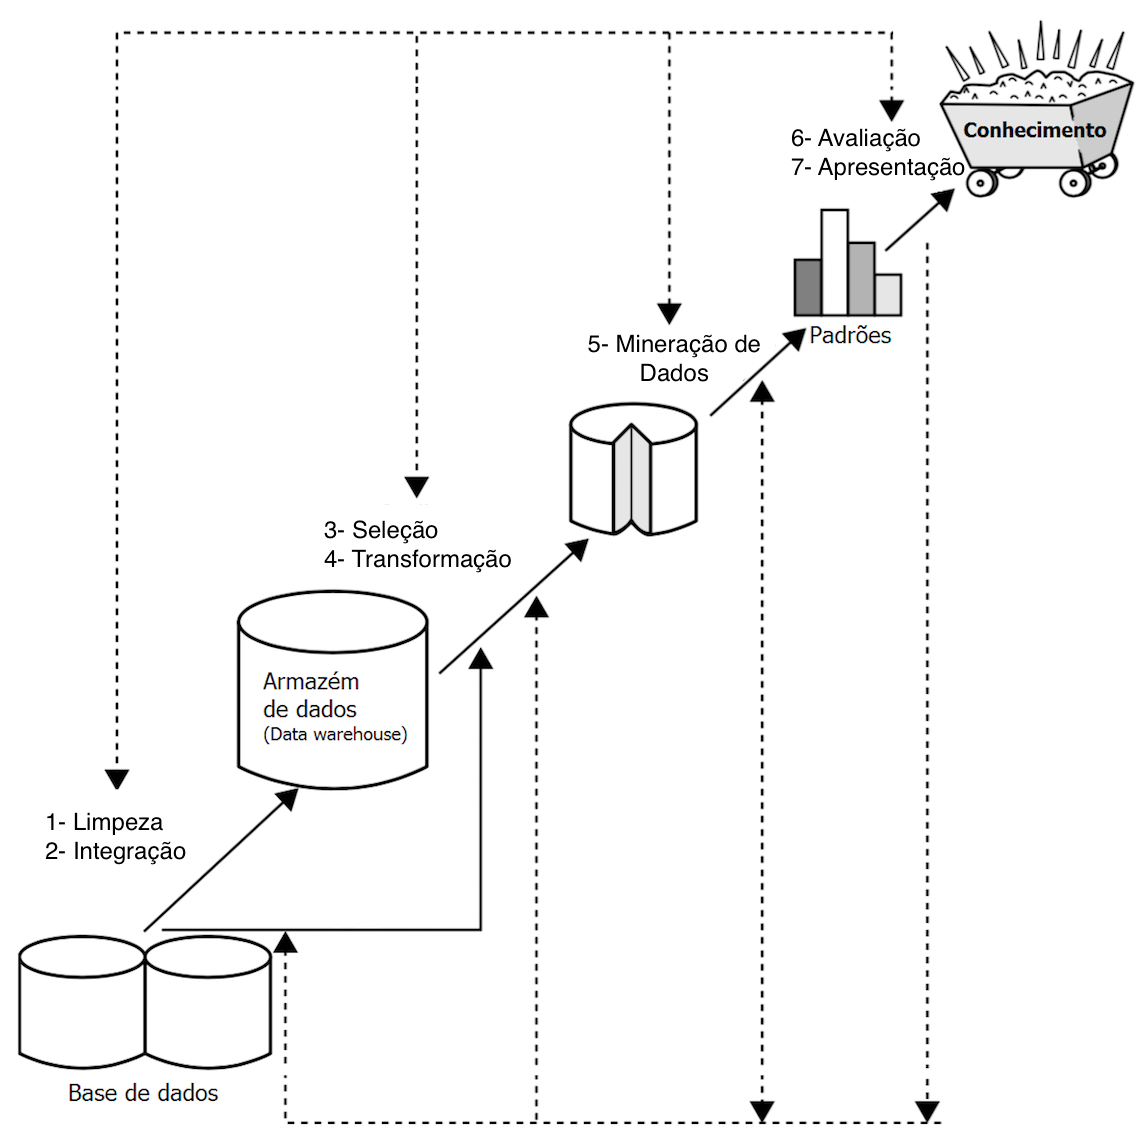
\includegraphics[width=1\textwidth]{Cap3/imagens/kdd2}
	\caption{Etapas do processo de KDD}
	\fonte{Adaptado de \citeonline{han}}
	\label{kdd-fig}
\end{figure}

\begin{enumerate}
	\item \textit{Data cleaning} (Limpeza de dados);
	\item \textit{Data integration} (Integração de dados);
	\item \textit{Data selection} (Seleção de dados);
	\item \textit{Data transformation} (Transformação de dados);
	\item \textit{Data mining} (Mineração de dados);
	\item \textit{Pattern evaluation} (Avaliação de padrões);
	\item \textit{Knowledge presentation} (Apresentação de conhecimento).
\end{enumerate}

É importante notar que algum dos processos acontecem na mesma etapa: Limpeza e integração; Seleção e transformação; Avaliação e apresentação.

De acordo com \apudonline{brachman}{fayyad2}, as etapas são interativas porque envolvem a cooperação da pessoa responsável pela análise de dados, cujo conhecimento sobre o domínio orientará a execução do processo. Por sua vez, a interação deve-se ao fato de que, com frequência, esse processo não é executado de forma sequencial, mas envolve repetidas seleções de parâmetros e conjuntos de dados, aplicações das técnicas de \textit{data mining} e posterior análise dos resultados obtidos, a fim de refinar os conhecimentos extraídos.

KDD refere-se ao processo global de descobrimento de conhecimento útil em bases de dados. \textit{Data mining} é um passo particular neste processo de aplicação de algoritmos específicos para extrair padrões (modelos) de dados. Os passos adicionais no processo KDD, como integração de dados, limpeza, seleção e transformação dos dados, assim como a interpretação e a apresentação dos resultados, asseguram que o conhecimento útil (informação) foi descoberto provenientes da etapa de mineração \cite{han}. A aplicação cega de métodos de \textit{data mining}, conforme alertado por \citeonline{navega}, pode ser uma atividade perigosa que conduz a descoberta de padrões sem sentido. 

O KDD evoluiu e continua evoluindo da interseção de pesquisas em campos como bancos de dados, aprendizado de máquinas (\textit{machine learning}), reconhecimento de padrões, estatísticas, inteligência artificial, aquisição de conhecimento para sistemas especialistas, visualização de dados, descoberta científica, recuperação de informação e computação de alto-desempenho. Aplicações de KDD incorporam teorias, algoritmos e métodos de todos estes campos \cite{credito-bancario}.

Apesar do conceito de \textit{data mining}, na maioria das vezes, ser utilizado pelas indústrias, mídias e centros de pesquisa para se referir ao processo de descoberta de conhecimento considerado em sua globalidade, o termo \textit{data mining} pode ser usado também para indicar o quinto estágio do KDD, sendo um processo essencial na descoberta e extração de padrões de dados. \citeonline{han}, adotam uma visão mais abrangente para a funcionalidade de mineração de dados: \textit{data mining} é o processo de descoberta de padrões interessantes e conhecimentos de um vasto conjunto de dados. A fonte dos dados pode ser banco de dados, \textit{data warehouses}, a Internet, outros repositórios de informações, ou dados correntes em sistemas dinâmicos.

Uma das definições, talvez, mais importante de \textit{data mining} foi elaborada por \citeonline{fayyad} "...o processo não-trivial de identificar, em dados, padrões válidos, novos, potencialmente úteis e ultimamente compreensíveis".

\textit{Data mining} ou mineração de dados, pode ser entendido então, como o processo de extrair informação, ou conhecimento útil, de algum conjunto de dados e utilizar este conhecimento adquirido para tomada de decisões ou descrever características e padrões descobertos \cite{conceito-data-mining}.

Diversos métodos são usados em \textit{data mining} para encontrar respostas ou extrair conhecimento interessante. Esses podem ser obtidos através dos seguintes métodos:

\begin{itemize}
	\item Classificação: associa ou classifica um item a uma ou várias classes. Os objetivos dessa técnica envolvem a descrição gráfica ou algébrica das características diferenciais das observações de várias populações. A ideia principal é derivar uma regra que possa ser usada para classificar, de forma otimizada, uma nova observação a uma classe já rotulada;
	
	\item Modelos de Relacionamento entre Variáveis: associa um item a uma ou mais variáveis de predição de valores reais, conhecidas como variáveis independentes ou exploratórias. Nesta etapa se destacam algumas técnicas estatísticas como regressão linear simples, múltipla e modelos lineares por transformações, com o objetivo de verificar o relacionamento funcional entre duas variáveis quantitativas, ou seja, constatar se há uma relação funcional entre X e Y;
	
	\item Análise de Agrupamento (\textit{Cluster}): associa um item a uma ou várias classes (ou \textit{clusters}). Os \textit{clusters} são definidos por meio do agrupamento de dados baseados em modelos probabilísticos ou medidas de similaridade. Analisar \textit{clusters} é uma técnica com o objetivo de detectar a existência de diferentes grupos dentro de um determinado conjunto de dados e, caso exista, determinar quais são eles;
	
	\item Sumarização: determina uma descrição compacta para um determinado subconjunto, por exemplos; medidas de posição e variabilidade. Nesta etapa se aplica algumas funções mais sofisticadas envolvendo técnicas de visualização e a determinação de relações funcionais entre variáveis. Estas funções são usadas para a geração automatizada de relatórios, sendo responsáveis pela descrição compacta de um conjunto de dados;
	
	\item Modelo de Dependência: descreve dependências significativas entre variáveis. Estes modelos existem em dois níveis: estruturado e quantitativo. O nível estruturado demonstra, através de gráficos, quais variáveis são localmente dependentes. O nível quantitativo especifica o grau de dependência utilizando alguma escala numérica;
	
	\item Regras de Associação: determinam relações entre campos de um banco de dados. Esta relação é a derivação de correlações multivariadas que permitam auxiliar as tomadas de decisão. Medidas estatísticas, como correlação e testes de hipóteses apropriados, revelam a frequência de uma regra no universo dos dados minerados;
	
	\item Análise de Séries Temporais: determina características sequênciais, como dados com dependência no tempo. Tem como objetivo modelar o estado do processo extraindo e registrando desvios e tendências no tempo. As séries são compostas por quatro padrões: tendência, variações cíclicas, variações sazonais e variações irregulares. Existem vários modelos estatísticos que podem ser aplicados a essas situações.
\end{itemize}

A maioria destes métodos são baseados em técnicas de aprendizado de máquina (\textit{machine learning}), reconhecimento de padrões e estatística. Essas técnicas vão desde estatística multivariada, como análise de agrupamentos e regressões, até modelos mais atuais de aprendizagem, como redes neurais, lógica difusa e algoritmos genéticos \cite{conceito-data-mining}.

Devido aos vários métodos estatísticos que são aplicados no processo de \textit{data mining}, \citeonline{fayyad} mostram uma relevância da estatística para o processo de extração de conhecimentos ao afirmar que essa ciência provê uma linguagem e uma estrutura para quantificar a incerteza resultante quando se tenta deduzir padrões de uma amostra a partir de uma população.

%%
% Machine Learning
%\section{\textit{MACHINE LEARNING}}\label{sec:machine-learning}
%Abstratamente, pode-se pensar em \textit{machine learning}, ou aprendizado de máquina, como um conjunto de ferramentas e métodos que tentam inferir padrões e extrair \textit{insights} de uma porção daquilo que se é observado no mundo. Por exemplo, ao tentar ensinar um computador a reconhecer os códigos postais escritos nos envelopes, os dados podem consistir em fotografias dos envelopes, além de um registro do código postal a que cada envelope estava endereçado, ou seja, dentro de um contexto, é possível selecionar um registro de ações de certos objetos, aprender com este registro e, em seguida, criar um modelo dessas atividades que irão informar a compreensão deste contexto futuramente \cite{machine-hacker}.
%
%Na prática, isto requer dados e, em aplicações atuais, isso, muitas vezes, significa uma grande quantidade de dados (talvez vários \textit{terabytes}). A maioria das técnicas de aprendizagem automática considera a disponibilidade de tais dados como algo inquestionável, o que significa novas oportunidades para a sua aplicação, em função da quantidade de dados que são produzidos como um produto de administrar companhias modernas.
%
%\textit{Machine learning} é a intersecção entre ciência da computação, engenharia, estatística e outras disciplinas. É possível ser aplicada em várias áreas, desde políticas a geociência. É uma ferramenta que pode ser utilizada para a solução de vários problemas. Qualquer campo que precisa interpretar e agir sobre dados pode se beneficiar do uso de técnicas de \textit{machine learning} \cite{machine-hacker}.
%
%A prática de engenharia está em utilizar a ciência para resolver um problema. Em engenharia, é comum resolver um problema determinista, em que a solução dada por humanos sempre resolve o problema. Se desenvolver um software para controlar uma máquina de venda automática é melhor que esta trabalhe sempre, independentemente do dinheiro depositado ou dos botões pressionados. Muitos problemas existem quando a solução não é determinista, isto é, ou não se sabe o suficiente sobre o problema ou não se tem poder computacional suficiente para delineá-lo adequadamente. Para esses problemas, precisa-se de estatísticas. 
%
%Uma das tarefas de \textit{machine learning} é a classificação. Na classificação, o trabalho é prever em que classe deve uma porção de dados ser enquadrada. Outra tarefa é a regressão que é a previsão de um valor numérico. Classificação e regressão são exemplos de aprendizado supervisionado, que são conhecidos como supervisionado, por dizer o que o algoritmo deve prever \cite{machine-learning}.
%
%O oposto de aprendizagem supervisionada é um conjunto de tarefas conhecidas como aprendizado não supervisionado, onde não há nenhum rótulo ou valor alvo dado para os dados. Uma solução para este tipo de aprendizagem é o agrupamento de itens semelhantes denominado de \textit{clustering}. Na aprendizagem não supervisionada, também pode-se querer encontrar valores estatísticos que descrevem os dados. Isso é conhecido como estimativa da densidade. Outra tarefa do aprendizado não supervisionado está em reduzir dados com várias funcionalidades até se chegar a um número reduzido, em que seja possível visualizá-lo em duas ou três dimensões \cite{machine-learning}.
%
%\subsection{\textit{Clustering}}
%A técnica de \textit{clustering} é um aprendizado não supervisionado que está presente em várias ferramentas de \textit{data mining}. Consiste na adoção de uma coleção de itens e, após particioná-los em pequenas coleções, conhecidos como \textit{cluster}, baseando-se em alguma heurística que será usada para comparar com outros itens da coleção.
%
%Técnicas para \textit{clustering} são partes fundamentais para um processo de mineração de dados. Uma implementação simples de \textit{clustering} pode criar experiências de usuário incrivelmente convincentes para alcançar resultados. Também pode ser aplicado a bases de texto utilizando algoritmos de \textit{text mining}, onde o algoritmo procura agrupar textos que falem sobre o mesmo assunto e separar textos de conteúdo diferentes.
%
%Por exemplo, caso queira considerar a localização geográfica dos contatos na rede \textit{Twitter}, é necessário realizar um \textit{cluster} nas conexões através de um determinado número de regiões com o intuito da melhor compreensão de oportunidades econômicas disponíveis.
%
%\subsection{Normalização de Dados}
%%Quando se recupera dados provenientes de uma API, é muito comum que esses não estarão no formato desejado para a sua análise. No caso do \textit{Twitter}, pode ser que usuários procurem por vagas de emprego escrevendo os nomes das vagas de alguma outra maneira sem ser o nome correto da vaga. Como exemplo, uma vaga para administrador de banco de dados pode ser buscado através da sigla "DBA", que em inglês significa \textit{Database Administrator}.
%
%A normalização de dados, procura então resolver esses problemas padronizando situações específicas que irá facilitar a análise posterior dos dados.
%
%\subsection{Computação de Similaridade}
%Após a normalização dos itens, é preciso verificar a similaridade entre eles. Podendo ser vagas de emprego, nomes de empresas, interesses profissionais, indicação geográfica, ou qualquer outro campo digitado na busca como um texto livre. Para isso é necessário definir uma heurística que conseguirá aproximar a similaridade entre dois valores quaisquer. Em algumas situações a similaridade heurística será um tanto óbvia, porém em outros casos será complicada. Por exemplo, comparar o tempo de carreira entre duas pessoas pode ser simples como uma operação de soma ou subtração. Mas comparar um elemento profissional, como "atitude de liderança" \space de uma maneira automatizada pode ser um desafio.

%%
% Python
\section{LINGUAGEM PYTHON}\label{sec:python}
Python é uma linguagem de programação orientada a objetos, interpretada e interativa. Incorpora módulos, excessões e de tipagem dinâmica alta. Possui uma sintaxe clara e simples, o que facilita o aprendizado para novos desenvolvedores, assim como a rápida leitura e interpretação para usuários mais experientes. Dispõe de interfaces para várias chamadas de sistemas (\textit{system calls}) e bibliotecas, também para vários sistemas de janelas, e é extensível a outras linguagens de programação como C ou C++. É também usada como uma linguagem de extensão para aplicações que precisam de uma interface programática \cite{python-doc}.

Outra característica da linguagem Python é a portabilidade, podendo ser utilizada em diversos sistemas operacionais como variantes do Unix, em sistemas Mac e também em PCs sob MS-DOS, Windows, Windows-NT, e OS/2.

É uma linguagem de programação de alto-nível que pode ser aplicada em soluções para diversas classes diferentes. Possui uma vasta quantidade de bibliotecas que atende a áreas como o processamento de \textit{strings} (expressões regulares, Unicode, cálculo de diferença entre arquivos), protocolos de Internet (HTTP, FTP, SMTP, XML-RPC, POP, IMAP, CGI \textit{programming}), engenharia de software (testes unitários, registro de logs, \textit{profiling}, análise de código Python), e interfaces para sistemas operacionais (\textit{system calls}, sistemas de arquivos, TCP/IP \textit{sockets}) \cite{python-doc}.

A sintaxe bastante expressiva e a abundância de suas bibliotecas tornam Python uma ótima linguagem para se obter resultados em várias questões. Algumas de suas utilidades são apresentadas conforme a seguinte lista:

\begin{itemize}
	\item Escrita de \textit{scripts}: Python é uma ótima linguagem para a criação de \textit{scripts}. É possível usar \textit{scripts} para analisar arquivos de texto, gerar amostra de entradas para testar programas, coletar conteúdos de páginas \textit{web} utilizando a biblioteca \textit{Beautiful Soup}, dentre outras atividades;
	\item Desenvolvimento \textit{backend} para aplicações \textit{web}: É possível criar APIs (\textit{Application Programming Interface}, apresentado no capítulo~\ref{ch:materiais-metodos}) e interagir com banco de dados. \textit{Frameworks} mais utilizados inclui \textit{Django}, \textit{Flask} e \textit{Pyramid};
	\item Análise e visualização de dados: Conforme o foco deste trabalho, bibliotecas como \textit{pandas}, \textit{NumPy} e recursos semelhantes a outras ferramentas como R e MATLAB estão dispostas através da biblioteca \textit{SciPy};
	\item \textit{matplotlib} e \textit{Seaborn}: são mecanismos que possibilitam a visualização dos dados.
\end{itemize}

A utilização dessa linguagem como ferramenta principal para este trabalho se justifica na utilização dos pacotes que facilitam a análise e interpretação de dados. Como exemplo, \textit{NumPy}, \textit{SciPy}, \textit{pandas}, \textit{matplotlib} e \textit{IPython} são os mecanismos indispensáveis para a mineração de informações juntamente com as estruturas de dados já presentes em Python como os \textit{dictionaries} (estruturas similares ao JSON), que permitem ordenar dados através de um modelo chave-valor. Devido então a sintaxe intuitiva que a linguagem possui e seu excelente ecossistema de bibliotecas, é possível acessar APIs e manipular dados com mais facilidade \cite{mining-social-web}.














\chapter{MATERIAIS E MÉTODOS}\label{ch:materiais-metodos}
Após a revisão bibliográfica de outros estudos e os fundamentos teóricos necessários para a mineração de dados utilizando Python, torna-se importante definir as ferramentas, tecnologias e procedimentos necessários para o desenvolvimento do projeto.

Este capítulo apresenta os materiais e métodos utilizados para a realização do processo de \textit{data mining}, onde, na seção~\ref{sec: tec-ferramenta} são apresentadas as tecnologias e ferramentas que serão utilizadas durante o estudo. Serão abordados quais as bibliotecas que a linguagem Python disponibiliza para a análise e mineração de dados e, também, como acessar a API do \textit{Twitter}. Esta será esclarecida também neste capítulo, após a explicação do conceito de API e o protocolo OAuth.

A seção~\ref{sec: metodologia} irá concluir o capítulo apresentando as etapas de \textit{data mining} com o intuito de evidenciar o processo para a obtenção de conhecimento útil.

\section{TECNOLOGIAS E FERRAMENTAS}\label{sec: tec-ferramenta}
Tecnologias e ferramentas para a implementação de \textit{scripts} e utilização dos algoritmos.

%% Bibliotecas Python
\subsection{Bibliotecas da Linguagem Python}\label{sec:bib_python}
Um dos grandes diferenciais da linguagem Python é o seu enorme conjunto de bibliotecas para soluções de diversos problemas.

A seguir serão apresentadas as bibliotecas necessárias para a mineração de dados, através das quais é possível coletar, limpar, transformar, realizar operações e apresentar resultados proveniente dos dados da rede social \textit{Twitter}. Para evitar repetições da palavra "biblioteca", o termo "pacote"\space também será utilizado com o mesmo significado no restante desta dissertação.
 
%%% sub: NumPy
\subsubsection{Biblioteca \textit{NumPy}}
\textit{NumPy} é o pacote fundamental para computação científica em Python. É o acrônico para \textit{Numerical Python}. Esta biblioteca provê:

\begin{itemize}
    \item \textit{ndarray} que é um objeto de matriz multidimensional;
    \item Funções que permitem realizar operações vetoriais ou operações matemáticas entre matrizes sem a necessidade de programar \textit{loops};
    \item Ferramentas para a leitura e escrita em conjuntos de dados matriciais;
    \item Operações de álgebra linear, transformada de Fourier e geração de números aleatórios;
    \item Ferramentas para a integração em outras linguagens de programação como C, C++ e Fortran.
\end{itemize}

Além da capacidade de rápido processamento em matrizes que o \textit{NumPy} oferece ao Python, um dos principais objetivos em relação a análise de dados é que serve como um "container"\space para os dados serem passado por algoritmos. Para dados numéricos, as matrizes de \textit{NumPy} são muito mais eficientes para a ordenação e manipulação de dados do que qualquer outra estrutura embutida em Python. Igualmente, bibliotecas escritas em linguagens de baixo nível, como C ou Fortran, podem operar dados gravados em matrizes da \textit{NumPy} sem precisar da cópia de qualquer dado \cite{python-analysis}.

A biblioteca \textit{NumPy} por si só, não provê uma funcionalidade de alto-nível para a análise de dados. Tendo um conhecimento sobre as matrizes de \textit{NumPy} e matrizes orientadas a computação (\textit{array-oriented computing}) irá facilitar o uso de outras ferramentas, como \textit{pandas}, com mais efetividade.

Para aplicações voltadas para a análise de dados, esta biblioteca possui grande funcionalidade em setores como:

\begin{itemize}
    \item Criação rápida de matrizes para a interação e limpeza de dados, separação e filtragem, transformação e outros tipos de operações computacionais;
    \item Algoritmos comuns para matrizes como ordenação, operações únicas e definidas;
    \item Eficiente descrição estatística e agregação/sumarização de dados;
    \item Alinhamento de dados e manipulação de dados relacionais para operações de junção e imerção (\textit{join} e \textit{merge}) de conjuntos de dados heterogeneos;
    \item Expressar lógicas de condições através de expressões matriciais ao invés de laços de repetições e condições como \textit{while, for, if-elif-else};
    \item Agrupamento de manipulação de dados (agregação, transformação, aplicação de funções).
\end{itemize}

Enquanto \textit{NumPy} oferece o fundamento computacional para essas operações, é preferível utilizar a biblioteca \textit{pandas} como base para a mineração de dados (especialmente de dados estruturados ou dados tabulados), devido a sua interface rica e de alto-nível no qual permite as tarefas com dados mais concisas e simples.

%%% sub: pandas
\subsubsection{Biblioteca \textit{pandas}}\label{pandas}
A biblioteca \textit{pandas} atrai o maior interesse de cientistas quanto a mineração de dados. Ela possui estruturas de dados de alto-nível e ferramentas de manipulação desenvolvidas para facilitar e agilizar a análise de dados em Python. \textit{pandas} é desenvolvida sob a biblioteca \textit{NumPy} e viabiliza o uso em aplicações centradas nesta. A seguir são expostas algumas soluções que a biblioteca disponibiliza \cite{python-analysis}:

\begin{itemize}
    \item Estrutura de dados com eixos rotulados suportam o alinhamento de dados automáticos ou explícitos. Isso evita erros comuns resultantes de dados desalinhados e dados indexados de formas diferentes provenientes de outras fontes de dados;
    \item A mesma estrutura de dados consegue manusear tanto dados de séries temporais como dados não-temporais;
    \item Operações e reduções aritméticas é passado para metadados (eixos rotulados);
    \item Manipulação flexível de dados em falta;
    \item \textit{Merge} (fundir) e outras operações relacionais encontradas em bancos de dados relacional.
\end{itemize}

Esta biblioteca possui duas estrutura de dados principais: \textit{Series} e \textit{DataFrame}. Estas estruturas não são uma solução universal para todos os problemas, mas provê uma base sólida e de fácil manipulação para a maioria das aplicações com mineração de dados.

Uma \textit{Series} é um tipo de \textit{array} ou uma matriz unidimensional, similar a um \textit{array} que possui uma matriz de dados (qualquer tipo de dado da biblioteca \textit{NumPy}) e um outro vetor associado a dados rotulados, chamados de \textit{index} (índice). Uma simples \textit{Series} é formado por uma única matriz de dados, conforme a Figura~\ref{pandas-series}.

\begin{figure}[h!]
	\centering
	\fbox{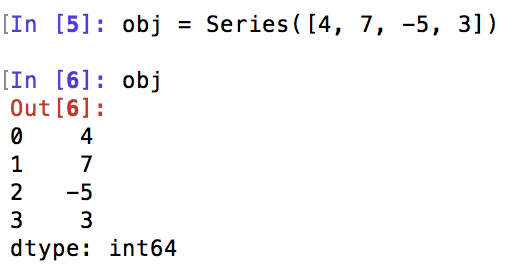
\includegraphics[width=.5\textwidth]{Cap4/imagens/pandas-series}}
	\vspace{0.1cm}
	\caption{Exemplo de uma \textit{Series}}
	\fonte{\citeonline{python-analysis}}
	\label{pandas-series}
\end{figure}

\textit{DataFrame} representa uma tabela, uma estrutura de dados do tipo planilha, que possui uma coleção ordenada de colunas, onde cada uma delas pode ter um tipo de valor diferente (numérico, \textit{string}, \textit{boolean}, etc.). O \textit{DataFrame} possui um índice para linhas e também para colunas. Pode ser interpretado como um dicionário de \textit{Series}. De uma maneira geral, o dado é armazenado como um ou mais blocos bi-dimensionais ao invés de uma lista, dicionário, ou outro tipo de coleção de matriz unidimensional \cite{python-analysis}.

Existem várias maneiras diferentes de se criar um \textit{DataFrame}, entretanto uma forma comum é um dicionário de dimensões iguais, conforme a Figura~\ref{pandas-dataframe} e a Figura~\ref{pandas-dataframe2}, ou uma matriz \textit{NumPy}.

\begin{figure}[h!]
	\centering
	\fbox{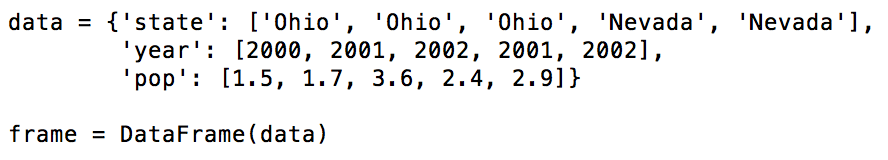
\includegraphics[width=.9\textwidth]{Cap4/imagens/pandas-dataframe}}
	\vspace{0.1cm}
	\caption{Criação de um \textit{DataFrame}}
	\fonte{\citeonline{python-analysis}}
	\label{pandas-dataframe}
\end{figure}

\begin{figure}[h!]
	\centering
    \fbox{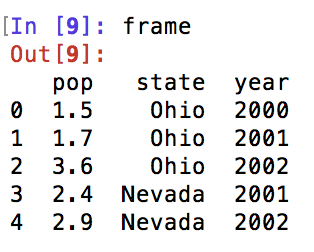
\includegraphics[width=.36\textwidth]{Cap4/imagens/pandas-dataframe2}}
    \vspace{0.1cm}
	\caption{Conteúdo de um \textit{DataFrame} pelo interpretador \textit{IPython}}
	\fonte{\citeonline{python-analysis}}
	\label{pandas-dataframe2}
\end{figure}

%%% sub: matplotlib
\subsubsection{Biblioteca \textit{matplotlib}}
O pacote \textit{matplotlib} é desenvolvido para a geração de gráficos bidimensionais a partir de \textit{arrays}. Gráficos comuns podem ser criados com alta qualidade a partir de simples comandos, inspirados nos comandos gráficos do MATLAB, exemplo ilustrado na Figura~\ref{matplotlib-fig}.

Quando usado em conjunto com ferramentas GUI (\textit{IPython}, por exemplo), esta biblioteca possui recursos interativos como zoom e visão panorâmica. Além disto, suporta várias ferramentas GUI \textit{backend}, nos diversos sistemas operacionais suportados pelo Python, e permitem exportar gráficos em diversos formatos: PDF, SVG, JPG, PNG, BMP, GIF, etc.

\textit{matplotlib} também possui várias ferramentas adicionais, como o \textit{mplot3d} para plotar gráficos tridimensionais, e o \textit{basemap} para mapeamentos e projeções.

\begin{figure}[h!]
  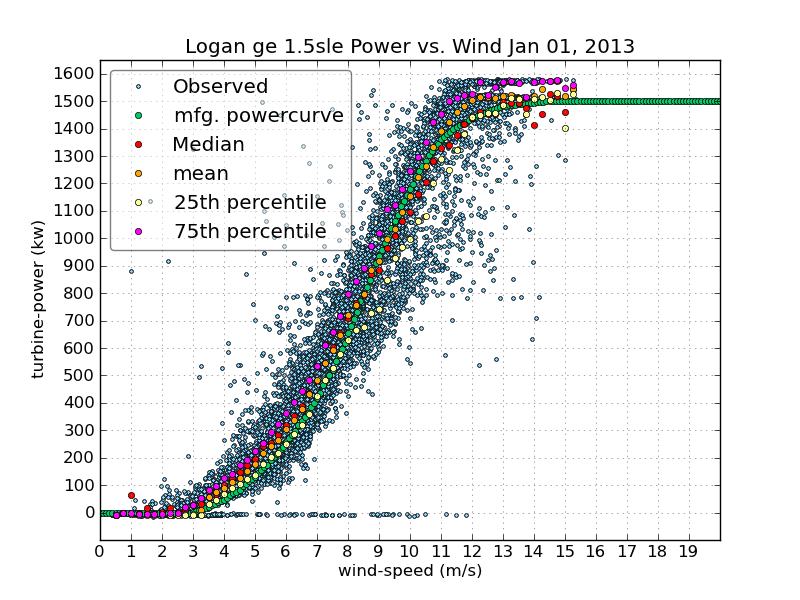
\includegraphics[width=1\textwidth]{Cap4/imagens/matplotlib}
  \caption{Exemplo de um gráfico gerado pelo \textit{matplotlib}}
  \fonte{\citeonline{matplotlib}}
  \label{matplotlib-fig}
\end{figure}


%%% sub: SciPy
\subsubsection{Biblioteca \textit{SciPy}}
\textit{SciPy} é uma coleção de pacotes que abordam uma série de soluções para diferentes domínios na computação científica. Na lista a seguir são apresentados exemplos desses pacotes \cite{python-analysis}:

\begin{itemize}
	\item \textit{scipy.integrate}: rotinas de integração numéricas e soluções de equações diferenciais;
	\item \textit{scipy.linalg}: rotinas de álgebra linear e decomposição de matrizes;
	\item \textit{scipy.optimize}: funções otimizadoras (minimizadoras) e algoritmos de busca em raíz;
	\item \textit{scipy.signal}: ferramentas para processamento de sinais;
	\item \textit{scipy.sparse}: matrizes esparsas e soluções de sistemas lineares esparsos;
	\item \textit{scipy.special}: agregador do \textit{SPECFUN}, uma biblioteca do Fortran que implementa várias funções matemáticas, como exemplo, a função gama;
	\item \textit{scipy.stats}: funções estatísticas, variáveis contínuas e discretas, testes estatísticos e outros modelos estatísticos;
	\item \textit{scipy.weave}: ferramenta para usar códigos \textit{inline} de C++ para acelerar a computação de matrizes.
\end{itemize}


%%% sub: IPython
\subsubsection{Interpretador \textit{IPython}}
O interpretador \textit{IPython} teve seu desenvolvimento iniciado em 2001, com o intuito de ser um interpretador interativo para a linguagem Python. Desde a sua criação o \textit{IPython} evoluiu grandemente, ao ponto de ser considerada uma das mais importantes ferramentas para computação científica em Python. Essa biblioteca não oferece nenhuma ferramenta para análise de dados ou análise computacional em si, sendo designada para maximizar a produtividade, tanto na interação computacional como no desenvolvimento de softwares. Oferece um fluxo de visualização de um modo \textit{execute-explore} ao invés do típico modelo \textit{edit-compile-run} de muitas outras linguagens de programação. Ela também provê uma pequena integração com o \textit{shell} e sistemas de arquivos. Como a maior parte da programação focada na mineração de dados envolve exploração, tentativa, erro e iteração, \textit{IPython}, em quase todos os casos, irá facilitar este tipo de trabalho \cite{python-analysis}.

\begin{figure}[h!]
  \centering
  \fbox{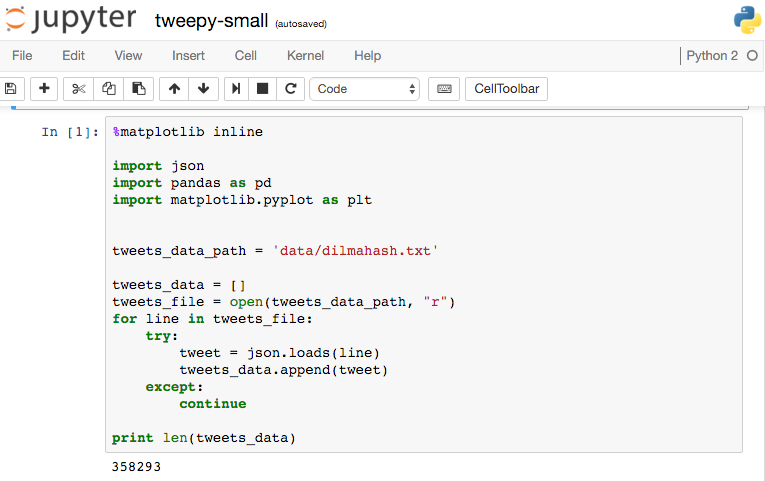
\includegraphics[width=0.95\textwidth]{Cap4/imagens/jupyter}}
  \vspace{0.1cm}
  \caption{Exemplo de uma página \textit{web} do \textit{IPython Notebook}}
  \fonte{Elaborado pelo autor}
  \label{ipython-fig}
\end{figure}

Hoje, o projeto \textit{IPython}, mantido pela empresa \textit{Jupyter}, engloba muito mais do que apenas um interpretador \textit{shell} para Python. Ele também inclui um console gráfico interativo, o \textit{IPython Notebook}, que provê ao usuário uma experiência de caderno (\textit{notebook-like}) através de um navegador \textit{web}, conforme Figura~\ref{ipython-fig}, e dispõe de um mecanismo de processamento paralelo. Assim como muitas outras ferramentas desenvolvidas para programadores, é extremamente customizável \cite{mining-social-web}.

%%% sub: Folium
\subsubsection{Biblioteca \textit{Folium}}
A linguagem Python possui a biblioteca \textit{Folium} que permite a visualização de dados em um mapa interativo desenvolvido em JavaScript o \textit{Leaflet}. \textit{Folium} permite que os dados de coordenadas sejam combinados com marcadores para a atribuição de informações ou notas em um mapa \cite{folium}.

A biblioteca possui integração com várias tecnologias que disponibilizam dados para a criação de mapas interativos, como \textit{OpenStreetmap}, \textit{MapQuest Open}, \textit{Mapbox} e \textit{Stamen} \cite{folium}.

%%% sub: NLTK
\subsubsection{Biblioteca \textit{NLTK}}
\textit{Natural Language Toolkit} - NLTK, é um conjunto de bibliotecas e programas para a representação simbólica e estatística do processamento de linguagem natural (NLP) para o Python \cite{nltk}.

A biblioteca NLTK se destina a apoiar a pesquisa e ensino em NLP ou areas correlativas incluindo linguagem empírica, ciência cognitiva, inteligência artificial, recuperação de informação e aprendizado de máquina. Permite o suporte a classificação, utilização de \textit{tokens}, \textit{stemming}, \textit{tagging}, análise (\textit{parsing}) e funcionalidades de raciocínio semântico \cite{nltk}.

Para a implementação de alguns códigos, esta biblioteca possibilitará a exclusão ou inclusão de certas palavras e símbolos durante a análise dos dados.

%%% sub: Word Cloud
\subsubsection{Biblioteca \textit{Word Cloud}}

\textit{Word Clouds}, conhecidas também como \textit{Tag Clouds}, são nuvens de palavras ou imagens formadas por um conjunto de palavras, utilizadas para apresentação e interpretação de palavras em um determinado texto.

Python possui uma biblioteca para a criação de \textit{Word Clouds}, em que, através de uma visualização, cada palavra tem seu tamanho regido pela relevância em determinado texto. Geralmente se trata de uma contagem simples das ocorrências de determinada palavra no texto \cite{citeword}.

%%
% API
\subsection{Interface de Programação de Aplicações - API}\label{subsec: api}
API é uma sigla para \textit{Application Programming Interface} e basicamente é uma tecnologia que permite um pedaço de \textit{software} se comunicar com outro pedaço de \textit{software}. Existem vários tipos de API e é comumente referenciado a outras tecnologias. Por exemplo, para o desenvolvimento deste trabalho será utilizado a API do \textit{Twitter}. 

Uma API é composta por uma série de funções acessíveis somente por programação, e que permitem utilizar características do \textit{software} menos evidentes ao utilizador tradicional. Neste caso, a rede social \textit{Twitter} possui vasta quantidade de dados, aonde através de sua API, permite que desenvolvedores externos possam implementar tecnologias que utilizam os seus dados.


%% 
% REST API
\subsubsection{Arquitetura REST}
Abreviação para Transferência de Estado Representacional (REST), é um estilo arquitetural baseado em recursos e nas representações desses recursos. Enfatiza a escalabilidade na interação entre componentes, a generalidade de interfaces, a implantação independente dos componentes de um sistema, o uso de componentes intermediários visando a redução na latência de interações, o reforço na segurança e o encapsulamento de sistemas legados. A REST ignora os detalhes da implementação de componente e a sintaxe de protocolo com o objetivo de focar nos papéis dos componentes, nas restrições sobre sua interação com outros componentes e na sua interpretação de elementos de dados significantes \cite{rest}.

REST foi um termo criado por \citeonline{rest}, onde ele modela um estilo de arquitetura para a construção de serviços \textit{web} consistentes e coesos. O estilo da arquitetura REST é baseado em recursos e nos estados desses recursos.

A funcionalidade de uma REST API é similar ao funcionamento de uma página \textit{web}, onde o usuário efetua uma requisição a um servidor \textit{web}, utilizando o protocolo HTTP, e recebe dados como resposta.

Um recurso é qualquer conteúdo ou informação que é exposto na Internet, podendo ser um documento, vídeo clip, até processos de negócio ou dispositivos. Para utilizar um recurso é necessário ser capaz de identificá-lo na rede e de ter meios para manipulá-lo. Tem-se então, o \textit{Uniform Resource Identifiers} (URI) para este propósito. Um URI unicamente identifica um recurso e, ao mesmo tempo, o torna endereçável ou capaz de ser manipulado utilizando um protocolo, como o HTTP. O URI de um recurso se distingue dos de qualquer outro recurso e é através do próprio URI que ocorrem as interações com o recurso \cite{rest-book}.

Recursos devem possuir pelo menos um identificador para ser endereçável, e cada identificador é associado com uma ou mais representações, que é uma transformação ou uma visão do estado do recurso em um instante de tempo. Essa visão é codificada em um ou mais formatos transferíveis, tal como XHTML, Atom, texto simples, XML, YML, JSON, JPG, MP3, entre outros  \cite{rest-book}.

Os recursos provêm o conteúdo ou objeto com o qual se quer interagir e para atuar sobre eles é utilizado os métodos de HTTP. Os métodos HTTP na arquitetura REST podem ser referenciados como Verbos, uma vez que representam ações sobre os recursos \cite{rest-book}.


\subsection{Protocolo de Autenticação - OAuth}
Protocolos de autenticação são capazes de, simplesmente, autenticar a parte que está se conectando, ou ainda de autenticar a parte que está conectando, assim como se autenticar para ele.

Neste trabalho será utilizado apenas o protocolo OAuth 1.0 para o acesso aos dados do \textit{Twitter}. É possível também, realizar a autenticação utilizando a versão mais atual, OAuth 2.0, mas será apenas referenciado, neste trabalho, para a melhor compreensão do funcionamento do protocolo.

OAuth é uma sigla para "\textit{open authorization}", ou autorização aberta, e provê um meio para que usuários autorizem uma aplicação acessar dados, com alguma finalidade, através de uma API, sem que os usuários precisem passar credenciais como nome de usuário e senha. De um modo geral, usuários são capazes de controlar o nível de acesso para estas aplicações e revogar este controle a qualquer momento \cite{mining-social-web}.

\subsubsection{Protocolo OAuth 1.0a}
OAuth 1.0a é um protocolo que permite que um cliente (\textit{client}) \textit{web} tenha acesso a um recurso protegido pelo seu dono em um servidor. Esta definição se dá através da RFC 5849. Que são documentos técnicos desenvolvidos e mantidos pelo Internet Enginnering Task Force (IETF), instituição que especifica os padrões que serão implementados e utilizados em toda a Internet.

A razão para a existência dessa tecnologia é para evitar problemas de usuários (donos dos recursos) compartilhar suas senhas com aplicações \textit{web}.

A versão OAuth 1.0a não permite que credenciais sejam trocadas utilizando uma conexão \textit{Secure Socket Layer} (SSL) através de um protocolo HTTPS. Por esse motivo, muitos desenvolvedores achavam tedioso o trabalho devido aos vários detalhes envolvidos em encriptação.

SSL é um padrão global para tecnologia de segurança. Tem como função principal criar um canal criptografado entre um servidor \textit{web} e um navegador (\textit{browser}) para garantir que todos os dados transmitidos sejam seguros e sigilosos.

Uma aplicação que está requerindo acesso é conhecida como \textit{client}, em alguns momentos chamado de \textit{consumer}, a rede social ou o serviço que contém os recursos protegidas é nomeado como \textit{server} (também chamado de \textit{provider}) e o usuário que concede o acesso é o \textit{resource owner} (dono do recurso, tradução livre). Com estes elementos, as três participações que envolvem o processo e a interação que estes elementos possuem é conhecida como \textit{"three-legged-flow"} ou de uma maneira mais coloquial, a \textit{OAuth dance}. Estas são as etapas fundamentais que envolvem a \textit{OAuth dance} que, como resultado, permite ao \textit{client} o acesso a recursos protegidos, conforme listado a seguir \cite{mining-social-web}:

\begin{enumerate}
	\item O \textit{client} obtém um \textit{token} de requisição do servidor de serviço (aplicação);
	\item O dono do recurso autoriza o \textit{token} de requisição;
	\item O \textit{client} troca o \textit{token} de requisição por um \textit{token} de acesso;
	\item O \textit{client} usa o \textit{token} de acesso para acessar os recursos protegidos com a consideração do dono do recurso.
\end{enumerate}

Para credenciais particulares, um \textit{client} começa com uma \textit{consumer key} e um \textit{consumer secret} e no fim do processo de \textit{OAuth dance}, termina com um \textit{token} de acesso e \textit{token} de acesso secreto que pode ser usado para acessar recursos protegidos.

\subsubsection{Protocolo OAuth 2.0}
Enquanto o protocolo OAuth 1.0a permite uma autorização útil para o acesso a aplicações \textit{web}, o OAuth 2.0 foi originalmente destinado a simplificar, significantemente, a implementação detalhada para desenvolvedores de aplicações \textit{web}, sendo fundamentado completamente no SSL para aspectos de segurança e para satisfazer uma vasta quantidade de casos de uso. Esses casos de uso variaram desde suporte para dispositivos móveis à necessidades empresariais e, consequentemente, às necessidades de um termo mais futuro, da "Internet das Coisas"\space \cite{mining-social-web}.

Diferentemente da implementação OAuth 1.0a, que consiste de um rígido conjunto de etapas, a implementação do OAuth 2.0, definido através do RFC 6749, pode variar de acordo com a particularidade do caso de uso. Um decorrer típico da execução do OAuth 2.0 tem a vantagem do SSL e, essencialmente, contém apenas poucos redirecionamentos que, acompanhada de em alto-nível, não possui tanta diferença em relação ao processo anterior que envolvem um ciclo do OAuth 1.0a.

%%
% Twitter
\subsection{Rede Social \textit{Twitter}}
Para definir o que seria o \textit{Twitter}, \citeonline{mining-social-web} aborda as seguintes necessidades que uma tecnologia social precisa disponibilizar à uma pessoa:

\begin{itemize}
	\item Permitir que a pessoa seja ouvida;
	\item Permitir que a pessoa satisfaça suas curiosidades;
	\item Permitir de um modo fácil e acessível;
	\item Permitir agora.
\end{itemize}

Essas observações são, de um modo geral, verdadeiramente humanas. Pessoas possuem o desejo de compartilhar ideias e experiências, que as permitam se conectar com outras pessoas, para serem ouvidas, e se sentirem parte ou digna de importância \cite{twitter2}.

Os dois últimos itens que \citeonline{mining-social-web} aborda ao comentar sobre as necessidades de uma tecnologia social, enfatizam a vontade de não ter alguma dificuldade para satisfazer as curiosidades ou realizar algum trabalho específico.

Uma maneira de descrever o \textit{Twitter} é, então, como um serviço de \textit{microblog} que permite uma breve comunicação entre pessoas. Mensagens de no máximo 140 caracteres explicam a "breve comunicação", que normalmente correspondem à pensamentos ou ideias sobre um determinado assunto, em outras palavras, \textit{Twitter} é um serviço global de trocas de mensagens, extremamente rápido e gratuito \cite{twitter1}.

Outro elemento interessante para a utilização dessa rede social é a assimetria ao "seguir" \space uma pessoa. Esta liberdade permite aos usuários atender as suas curiosidades. Diferentemente de outras redes sociais, como \textit{Facebook} e \textit{LinkedIn}, que requer uma aceitação mútua da conexão entre os usuários, o modelo de relacionamento no \textit{Twitter} viabiliza os acontecimentos de qualquer outro cliente na rede, podendo ser alguma especulação sobre celebridades, atualizações sobre times de esportes, algum tópico particular político ou o simples desejo de se conectar a alguém \cite{twitter2}.


\subsubsection{API do \textit{Twitter}}\label{api-twitter}
\textit{Twitter} é caracterizado como um serviço de \textit{microblog} em tempo real, que permite os usuários postarem pequenas atualizações de qualquer situação que desejar, essas postagens são chamados de \textit{tweets}, que aparecem em \textit{timelines} (linhas de tempo). \textit{Tweets} podem incluir uma ou mais entidades em seus 140 caracteres de conteúdo e referenciar um ou mais lugares que mapeiam localizações do mundo real \cite{mining-social-web}.

%É necessário ter um entendimento sobre usuários (\textit{users}), \textit{tweets} e \textit{timelines} para o uso efetivo da API do \textit{Twitter}. Será, então, abordado uma breve explicação sobre a plataforma de objetos do \textit{Twitter}, com o intuito de interagir com a sua API para a coleta de dados \cite{twitter-doc}.

A essência do \textit{Twitter} são os \textit{tweets} e, apesar deles serem representados como 140 caracteres de conteúdo textual associado a uma atualização de um usuário, existe muito mais informação através dos metadados. Em adição ao conteúdo textual de um \textit{tweet}, eles vêm empacotados em dois pedaços de metadados: entidades e lugares. Entidades de um \textit{tweet} são, basicamente, menções de usuários, \textit{hashtags}, URLs e mídias que são associadas a um \textit{tweet}. Lugares são localizações no mundo real, que podem estar adjunto a um \textit{tweet}. Um lugar pode ser uma localização atual aonde o \textit{tweet} foi composto, mas também pode ser uma referência a algum lugar descrito no \textit{tweet} \cite{twitter-doc}.

Para exemplificar, considere o \textit{tweet} apresentado pela Figura~\ref{fig:tweet}. O \textit{tweet} possui 83 caracteres (incluindo espaços e quebra de linhas) e contém quatro entidades: duas \textit{hashtags} \#GameOfThrones e \#Linux, uma menção ao usuário @itsfoss e uma imagem como conteúdo de mídia. Não existe porém, uma localidade exposta nesta postagem, porém existe muito mais informações no metadado deste \textit{tweet} que demonstra a quantidade de dados que se pode coletar.

\begin{figure}[h]
  \centering
  \fbox{
\includegraphics[width=0.8\textwidth]{Cap4/imagens/tweet}}
  \vspace{0.1cm}
  \caption{Exemplo de um \textit{tweet}}
  \fonte{\citeonline{twitter-example}}
  \label{fig:tweet}
\end{figure}


\textit{Timelines} são coleções de \textit{tweets} ordenadas cronologicamente. É possível afirmar, que \textit{timeline} é qualquer coleção específica de \textit{tweets} apresentadas em uma ordem cronológica. Através da perspectiva de um usuário do \textit{Twitter}, a \textit{timeline} inicial (\textit{home}) é a visualização principal quando este usuário acessa a sua conta no serviço do \textit{Twitter} \cite{mining-social-web}. Quando este acesso é realizado, normalmente acontece através do endereço https://twitter.com. A URL para a \textit{timeline} de algum usuário em particular, no entanto, precisa ser sufixado com o contexto que identifica este usuário específico, por exemplo; https://twitter.com/unixstickers.

A figura~\ref{fig:tweet-deck} ilustra a aplicação \textit{TweetDeck} que disponibiliza a customização da visualização de várias \textit{timelines}.

\begin{figure}[h]
  \centering
  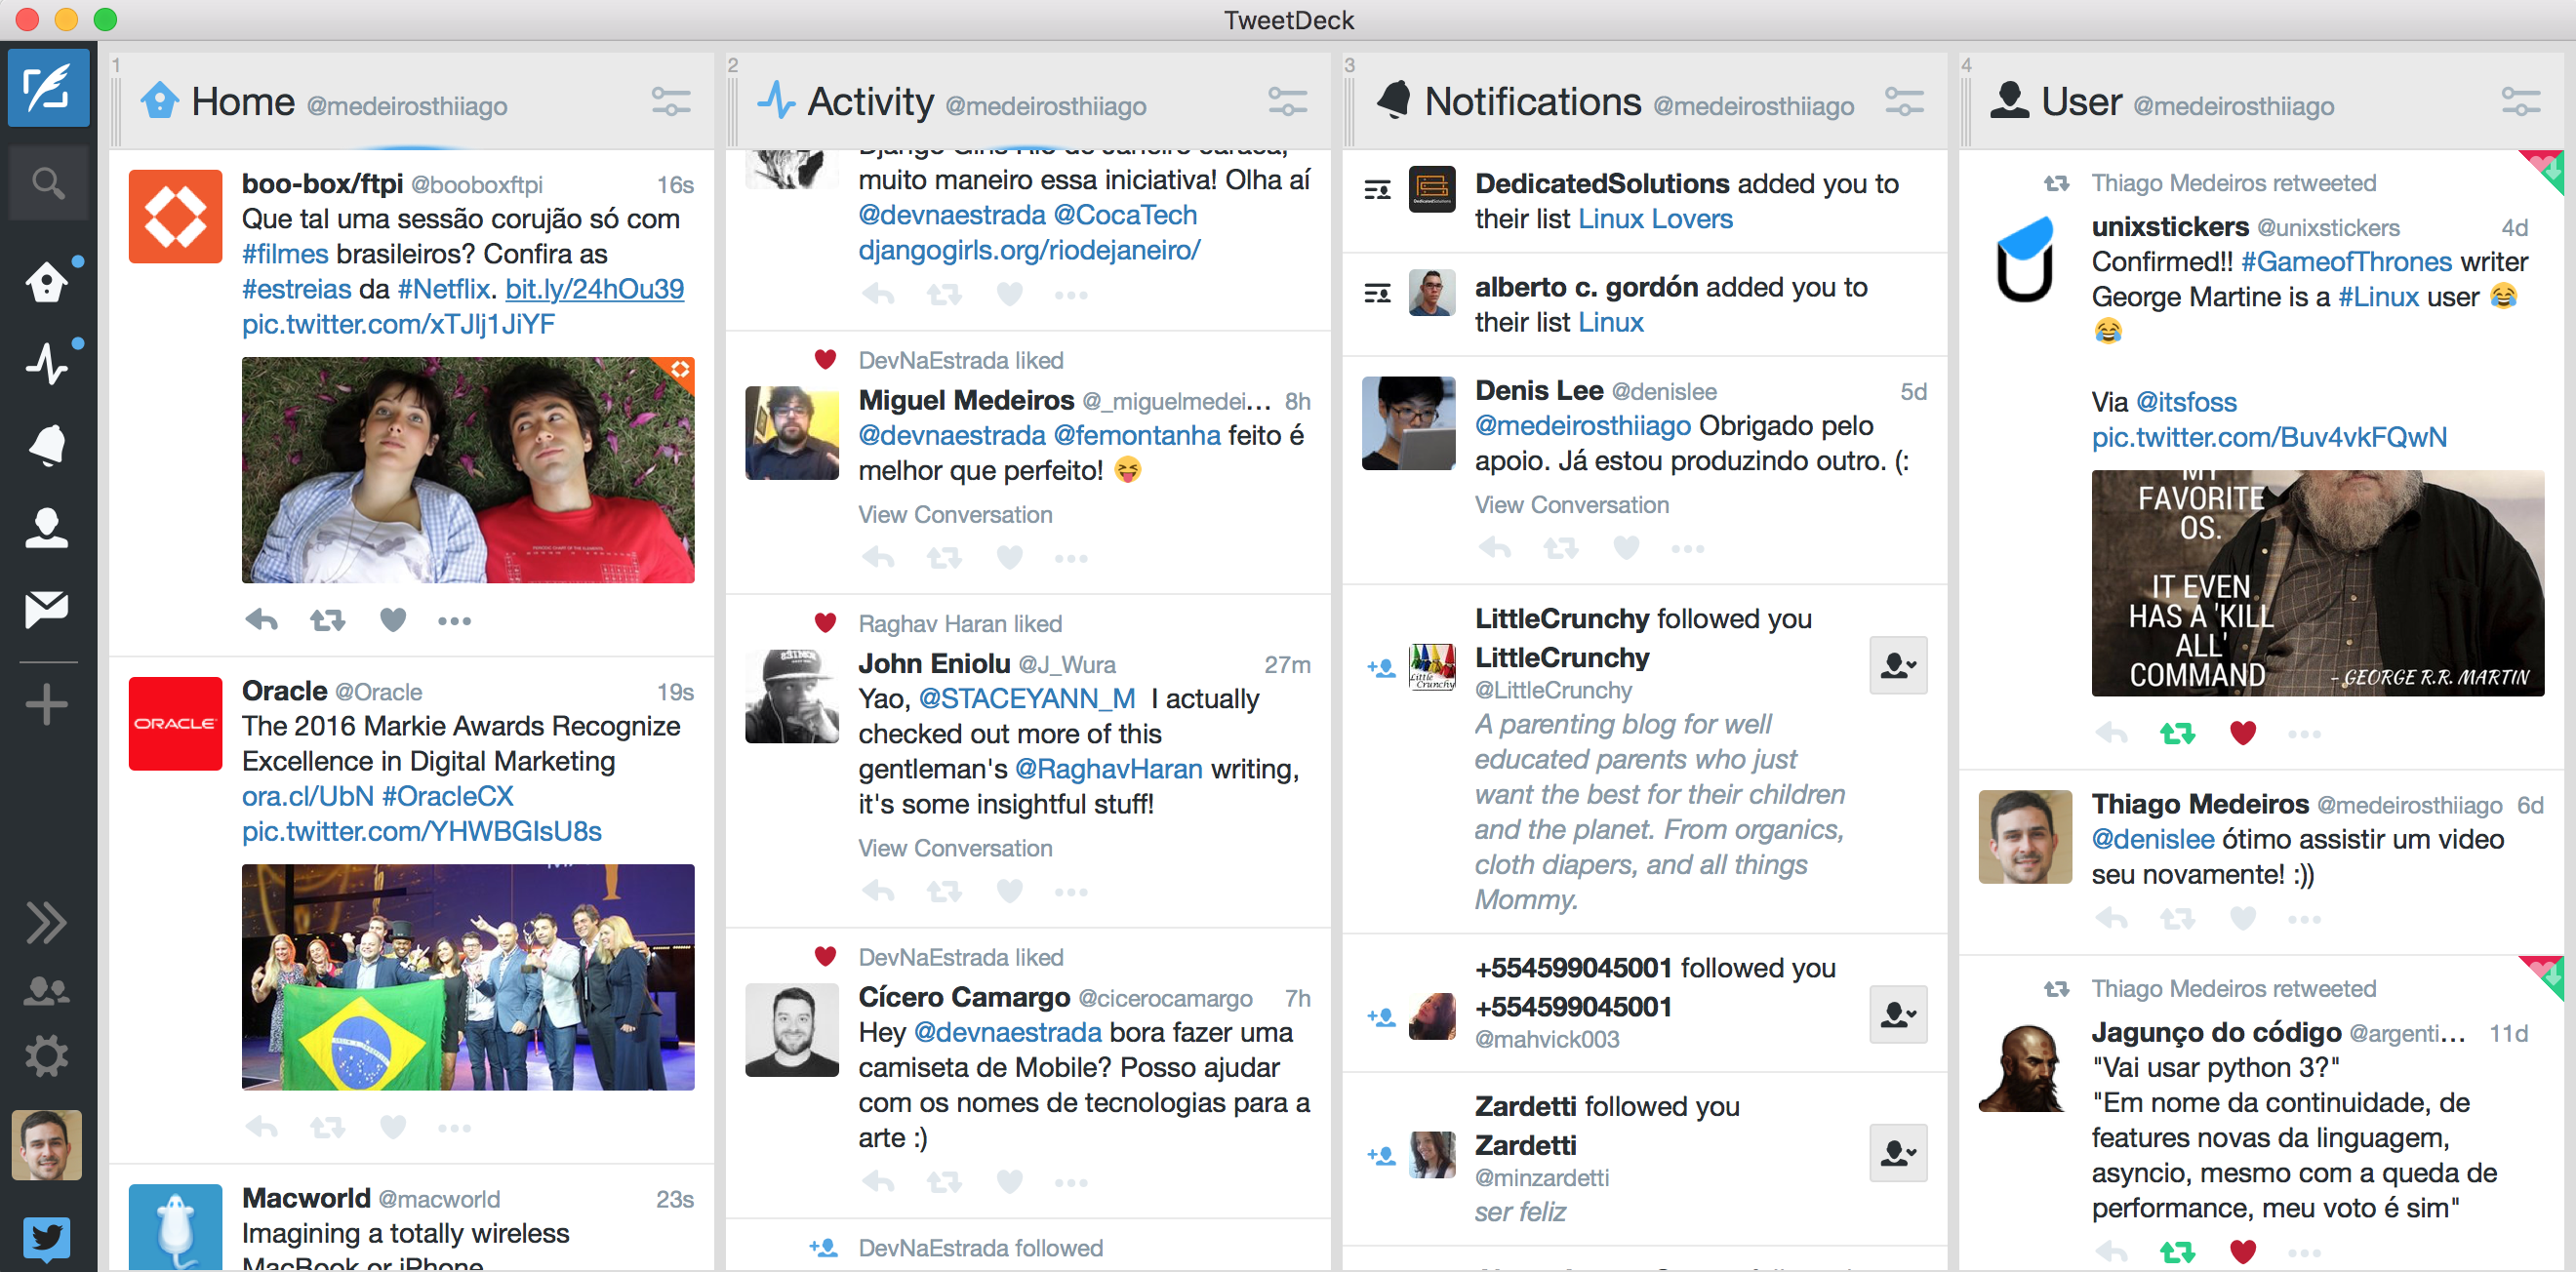
\includegraphics[width=1\textwidth]{Cap4/imagens/tweet-deck}
  \caption{Aplicação \textit{TweetDeck} apresentando várias \textit{timelines}}
  \fonte{Elaborado pelo autor}
  \label{fig:tweet-deck}
\end{figure}

%\textbf{\textcolor{red}{[MELHORAR]}} Enquanto \textit{timelines} são coleções de \textit{tweets} com uma velocidade relativamente baixa de atualizações, \textit{streams} são amostras de \textit{tweets} públicos fluindo através do \textit{Twitter} em tempo real. Uma ferramenta pública que a rede social disponibiliza é o \textit{firehose}, que permite coletar, ou visualizar, centenas de milhares de \textit{tweets} por minuto durante eventos com interesses bem abrangentes, como debates presidenciais, finais de campeonatos esportivos e outros acontecimentos que engloba milhares de internautas \cite{twitter-doc}.

\textit{Twitter} possui três tipos de APIs que permitem que desenvolvedores acessem seus dados, isto é, são capazes de coletar, ou consumir, \textit{tweets} completos, entidades específicas e também informações dos usuários ou réplicas de mensagens.

A API de busca do \textit{Twitter} (\textit{Twitter's Search API}), tem a funcionalidade de capturar dados através de uma busca ou um usuário. Esta API permite o acesso a dados que já existem em \textit{tweets} previamente publicados. Através da API de busca, o usuário solicita \textit{tweets} que correspondem a algum critério de busca, podendo ser nome de usuários, localizações, nome de lugares, palavras-chaves e \textit{hashtags} \cite{twitter-doc}.

Através da API de busca, desenvolvedores podem coletar \textit{tweets} que ocorreram e são limitados a um resultado de 3200 publicações dependendo do critério de busca. Utilizando uma \textit{hashtag} específica a API permite coletar até 5000 \textit{tweets} por \textit{hashtag}. Estas limitações acontecem em um determinado período de tempo, onde hoje, são permitidos 180 requisições a cada 15 minutos \cite{twitter-doc}.

A segunda tecnologia, e também a tecnologia utilizada neste trabalho para a coleta dos dados, é a API de \textit{streaming} do \textit{Twitter} (\textit{Twitter's Streaming API}) onde se comporta de maneira diferente da API de busca. Nesta, é recebido dados que estão acontecendo em tempo real. Através da API de \textit{streaming}, é possível registrar um conjunto de critérios de busca, para que cada vez que um \textit{tweet} corresponder ao critério salvo, irá ser enviado diretamente ao seu solicitante \cite{twitter-doc}.

A principal desvantagem da API de \textit{streaming} é que o \textit{Twitter} provê apenas uma parte das publicações que estão acontecendo. E então, a porcentagem dos \textit{tweets} coletados por esta API variam de acordo com o número de requisições de usuários durante o tráfego de dados naquele exato momento. A razão por não receber todas as publicações é porque o \textit{Twitter} precisa dispor de uma infraestrutura que suporte todas as requisições dos \textit{tweets} que estão sendo publicados \cite{twitter1}.

O \textit{Twitter Firehose} é a última API disponibilizada e funciona semelhante a API de \textit{streaming}, onde é enviado a usuários finais os dados de \textit{tweets} que são publicados em tempo real. A diferença é que o \textit{Twitter Firehose} garante o consumo de 100\% dos \textit{tweets} que correspondem ao critério de busca \cite{twitter-doc}.

A API de \textit{Firehose} é mantida por dois provedores de dados, GNIP e DataSift, que possuem relações empresarias com o \textit{Twitter}. Devido a esta relação e a disponibilidade de infraestrutura destas empresas, a utilização do \textit{Firehose} não é gratuita mas também exclui várias restrições de usos impostas pelo \textit{Twitter}, diferentemente da API de \textit{streaming} onde é possível realizar a coleta sem custos \cite{twitter1}.

% Bibliotecas Twitter
\subsubsection{Bibliotecas Para o Consumo de Dados da API do \textit{Twitter}}
O acesso a API acontece através da criação de uma aplicação pela página \textit{web} de desenvolvimento do \textit{Twitter}, https://apps.twitter.com. Após a criação desta aplicação é fornecido ao usuário informações para o acesso utilizando o protocolo OAuth. Será informado uma chave exclusiva da API da aplicação, uma chave secreta, o \textit{token} de usuário OAuth e credenciais secretas do usuário OAuth \cite{mining-social-web}.

Com estas credencias é possível, então, ter acesso as APIs do \textit{Twitter} e, consequentemente, o que a mesma disponibiliza para os usuários. Para o consumo desta API, a linguagem de programação Python apresenta algumas bibliotecas que facilita este tipo de serviço, listadas a seguir:

\begin{itemize}
	\item \textit{requests-oauthlib};
	\item \textit{tweepy};
	\item \textit{python-twitter};
	\item \textit{oauthlib}.
\end{itemize}

A biblioteca \textit{tweepy}, será a mais utilizada para as implementações deste trabalho devido a fácil interação com a APIs do \textit{Twitter}. Esta biblioteca permite o acesso a todos os métodos presentes na API, cada método pode aceitar parâmetros diversos e retornar respostas quando invocados \cite{tweepy}.

O Código~\ref{cod:exempla-api} exemplifica o consumo da API segundo \citeonline{tweepy}.

\lstinputlisting[language=Python, label=cod:exempla-api, caption=Acesso à API do \textit{Twitter}]{Cap4/src/acesso.py}

Quando um método da API é invocado, quase todos os seus retornos serão uma instância de um modelo \textit{tweepy}. Este modelo irá conter dados retornados do \textit{Twitter} onde é possível manipulá-los da maneira como o programador preferir \cite{tweepy}.


%%
% METODOLOGIA
\section{METODOLOGIA E DESENVOLVIMENTO}\label{sec: metodologia}
Um trabalho científico, segundo \citeonline{demo}, pode ser avaliado pela sua qualidade política e pela sua qualidade formal. A qualidade política é referenciada pelos seus conteúdos, relevância e utilidade prática. Já a qualidade formal, diz respeito aos meios e formas usados na produção do trabalho, referindo-se ao domínio de técnicas de coleta e interpretação de dados, manipulação de fontes de informação, conhecimento demonstrado na apresentação do referencial teórico e apresentação escrita ou oral em conformidade com os ritos acadêmicos \cite{metodologia}.

A característica política deste trabalho se dá com a demonstração da possibilidade de utilização da linguagem Python para a mineração de dados em redes sociais, especificamente neste presente trabalho o \textit{Twitter}, através das APIs disponibilizadas por este.

Para o cumprimento das qualidades citadas, desempenhou-se uma pesquisa científica em que segundo \citeonline{goldenberg}, precisa satisfazer os seguintes requisitos:

\begin{enumerate}
	\item a existência de uma pergunta que se deja responder;
	\item a elaboração de um conjunto de passos que permitam chegar à resposta;
	\item a indicação do grau de confiabilidade na resposta obtida.
\end{enumerate}

A pergunta a ser respondida diz respeito da viabilidade de utilizar Python como uma ferramenta útil para a mineração de dados e, consequentemente, a apresentação dos resultados obtidos. Sendo necessário o conhecimento teórico sobre técnicas de mineração de dados e das funcionalidades e bibliotecas que a linguagem em estudo dispõe.

Para o cumprimento do segundo requisito de \citeonline{goldenberg}, foram desenvolvidos \textit{scripts} para a autenticação, coleta e limpeza de dados utilizando o modelo Iterativo e Incremental como técnica de Engenharia de \textit{Software}.

O desenvolvimento Iterativo e Incremental é um modelo clássico para o processo de criação de \textit{softwares}, que utiliza padrões do modelo \textit{Rational Unified Process} - RUP e também de desenvolvimentos ágeis, tem como característica o retrabalho em que o tempo de revisão e melhorias de partes dos \textit{scripts} é pré-definido e o planejamento estagiado em que várias partes do \textit{script} são desenvolvidos em paralelo e integrados quando completos \cite{rup}.

A apresentação dos resultados e, também, o indicativo da resposta alcançada pela mineração dos dados, ocorreu através da implementação de códigos Python que resultaram em informações interpretadas através de gráficos, imagens e mapa.

O presente trabalho se caracteriza, também, segundo \citeonline{gil}, como uma pesquisa exploratória, em que visa proporcionar familiaridade com problema ou necessidade e torná-lo explícito ou também a construção de hipóteses. Através da interpretação dos dados minerados é possível a explicitação e o desenvolvimento de hipóteses apresentadas pelas publicações na rede social \textit{Twitter}.














\chapter{IMPLEMENTAÇÃO DAS TÉCNICAS E ANÁLISE DOS RESULTADOS}\label{ch:implementacao}

Este capítulo tem como finalidade apresentar com um maior nível de detalhamento as técnicas utilizadas neste trabalho, com o objetivo de se atingir as metas propostas já descritas no Capítulo~\ref{ch:introducao}, no item~\ref{sec:objetivos}.

\section{COLETA DE DADOS}
Uma característica comentada anteriormente sobre a rede social \textit{Twitter} é a disponibilidade de informações de eventos em tempo real. Os \textit{tweets} podem ser postados com o intuito de comentar sobre a final de um campeonato de futebol, datas importantes, acontecimentos internacionais e políticos, entre outros.

Para este trabalho foi aproveitado o dia 17 de abril de 2016, onde foi realizado a votação do Congresso Brasileiro pela continuação do processo de Impeachment do cargo de presidente da senhora Dilma Rouseff. Neste dia milhares de \textit{tweets} foram publicados utilizando a \textit{hashtag} \#ImpeachmentDay com o objetivo de comentar sobre o evento de votação e, também, a atual situação política do Brasil.

Com a finalidade de coletar todos os dados da referida \textit{hashtag}, foi desenvolvido um \textit{script} que utiliza o serviço de \textit{Stream} do \textit{Twitter}, também conhecido como \textit{FireHose}.

As primeiras linhas do Código~\ref{coleta-script} servem para importar as bibliotecas e objetos necessários para a utilização da API do \textit{Twitter}, assim como as informações das chaves de acesso e \textit{tokens} para o protocolo OAuth, que são fundamentais para a comunicação com o serviço de \textit{Stream}.

\lstinputlisting[language=Python, label=coleta-script, caption=\textit{Script} coletar-hashtags.py]{Cap5/src/coletar-hashtags.py}

A partir da linha 11 é criado uma classe que instancia um serviço de escuta para este \textit{Stream}. O serviço de escuta é responsável por observar todos os \textit{tweets} que são publicados e após identificar no \textit{tweet} alguma palavra ou a \textit{hashtag} semelhante a palavra declarada na linha 28, é então capturado e impresso na tela de execução do \textit{script}.

Quando este \textit{script} está em execução é mostrado na tela todos os \textit{tweets} que estão sendo coletados, já filtrados, porém não está sendo persistido em nenhum arquivo ou banco de dados. Com o intuito de salvar todos estes dados foi utilizado o comando \textit{stdout} ($>$), presente em sistemas operacionais de base \textit{Unix}. O comando \textit{stdout} permite redirecionar a saída do código anterior, no caso a execução do \textit{script} coletar-hashtags.py, para um novo arquivo ou um arquivo já existente conforme ilustrado pela Figura~\ref{exec-coleta}.

\begin{figure}[h]
	\centering
	\fbox{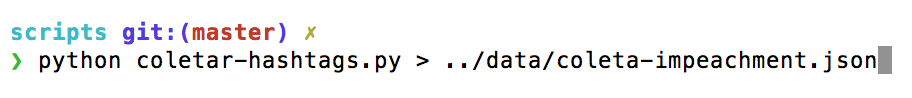
\includegraphics[width=0.95\textwidth]{Cap5/imagens/execucao-script}}
	\caption{Execução do \textit{script} para coleta de dados}
	\vspace{-0.3cm}
	\legend{FONTE: Elaborado pelo autor}
	\label{exec-coleta}
\end{figure}

O \textit{script} apresentado no Código~\ref{coleta-script} permaneceu em execução durante 14 horas (das 08:30 às 22:30) do dia 17 de abril, concluindo em um arquivo de 2.6 gigabytes. O formato deste arquivo é um JSON onde apresenta todas as informações presentes em um \textit{tweet}, demonstrado através do Código~\ref{peda-json}.

\lstinputlisting[language=Python, label=peda-json, caption=Exemplo de um \textit{tweet} no formato JSON]{Cap5/src/peda.json}

\section{ANÁLISE DE DADOS}
Após a coleta de dados foi gerado, então, um arquivo JSON de 2.6 gigabytes. Portanto a próxima etapa será analisar estes dados para extrair informações úteis.

Foi realizado testes no arquivo JSON coletado para verificar se existe algum tipo de \textit{dirty data}, que são informações quebradas, dados irrelevantes ou códigos que impedem a execução de \textit{scripts} de mineração \cite{dirty-data}. A Figura~\ref{fig-dirty} demonstra o único padrão de \textit{dirty data} encontrado dentro do arquivo.

\begin{figure}[h]
	\centering
	\fbox{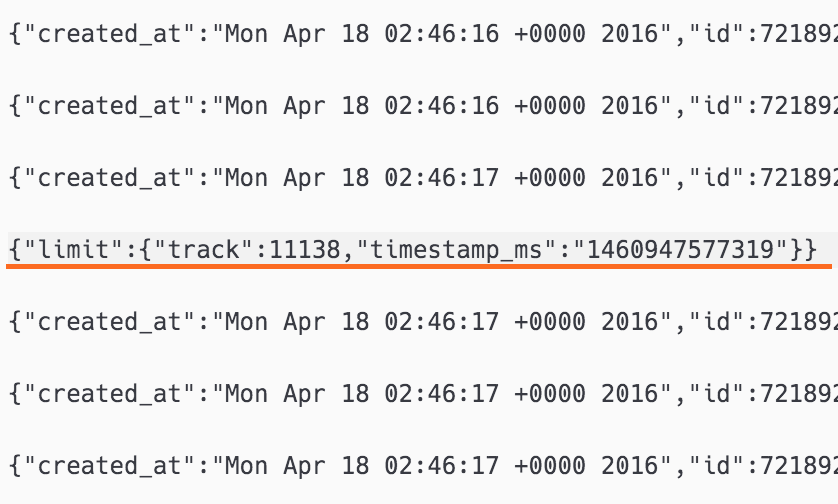
\includegraphics[width=0.95\textwidth]{Cap5/imagens/limit}}
	\caption{\textit{Dirty Data} presente no arquivo coletado}
	\vspace{-0.3cm}
	\legend{FONTE: Elaborado pelo autor}
	\label{fig-dirty}
\end{figure}

Dentro das milhares linhas do arquivo, existem algumas linhas contendo este mesmo padrão ("limit":), que foram removidos utilizando outra ferramenta de sistemas baseados em Unix, o \textit{grep}.

A ferramenta \textit{grep} é considerada um "canivete suíço" \space para o uso de expressões regulares e possui uma funcionalidade que permite realizar uma consulta inversa, ou seja, o usuário passa um padrão ou uma palavra que se deseja encontrar dentro de um determinado arquivo, e após encontrar todas as ocorrências, o \textit{grep} seleciona tudo o que não contém este padrão ou palavra.

Combinado com o comando de \textit{stdout} ($>$), é possível redirecionar todos os dados que não possui este tipo de \textit{dirty data} para um novo arquivo conforme a Figura~\ref{limpa-dado}.

\begin{figure}[h]
	\centering
	\fbox{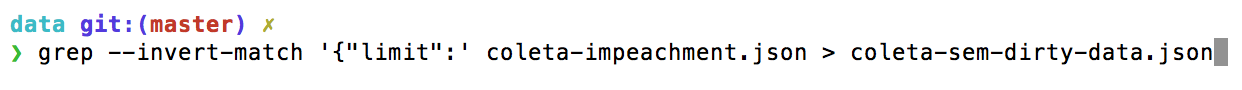
\includegraphics[width=0.95\textwidth]{Cap5/imagens/grep}}
	\caption{Utilizando o comando \textit{grep} para gerar um novo arquivo sem \textit{dirty data}}
	\vspace{-0.3cm}
	\legend{FONTE: Elaborado pelo autor}
	\label{limpa-dado}
\end{figure}

Tendo então um arquivo JSON sem a presença de \textit{dirty data} é possível iniciar o processo de extração de conhecimento utilizando o interpretador \textit{IPython}.

Nesta primeira etapa é importado as bibliotecas necessárias para se trabalhar com arquivos do tipo JSON e também para a geração de gráficos, conforme o Código~\ref{ini-py}.

\lstinputlisting[language=Python, label=ini-py, caption=Leitura do arquivo JSON]{Cap5/src/ini.py}

A primeira linha do Código~\ref{ini-py} permite a visualização de gráficos e planilhas no \textit{IPython}. A partir da linha 8, é realizado a construção de um \textit{DataFrame}, que é definido na seção~\ref{pandas}, através leitura do arquivo coleta-sem-dirty-data.json.

A execução deste código permite, então, gerar um \textit{DataFrame} e informar o número de \textit{tweets} que ele contém. Esses \textit{DataFrames} possuem uma arquitetura semelhante ao formato de tabelas em que é possível adicionar uma coluna ou uma tabela a uma variável em Python. Através do mapeamento de uma condição específica em um \textit{DataFrame}, apresentado no Código~\ref{map-lingua} para mapear o texto, a língua e o país em que o \textit{tweet} foi publicado.

\lstinputlisting[language=Python, label=map-lingua, caption=Mapeamento de variáveis para um \textit{DataFrame}]{Cap5/src/map-lingua.py}

Após o mapeamento das informações do \textit{DataFrame} foi construído um gráfico em barras que indica as quantidades de \textit{tweets} em relação as quatro línguas mais significativas no conjunto de dados coletados. A Figura~\ref{lingua} apresenta o gráfico gerado.

\begin{figure}[h]
	\centering
	\fbox{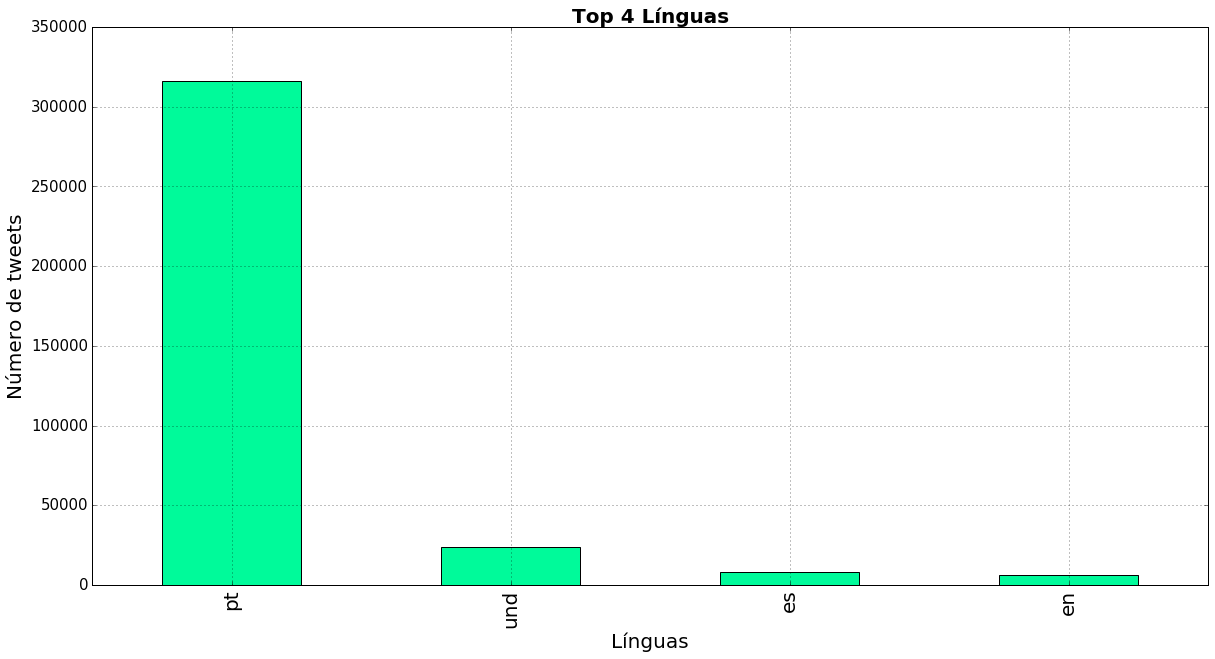
\includegraphics[width=1\textwidth]{Cap5/graficos/linguas}}
	\caption{Línguas que mais realizaram \textit{tweets}}
	\vspace{-0.3cm}
	\legend{FONTE: Elaborado pelo autor}
	\label{lingua}
\end{figure}

É possível verificar nesta figura que existe uma barra com o nome de \textit{und} para especificar a segunda língua que realizou mais \textit{tweets}. Essa é uma condição em que não foi identificada a língua de origem e então a API do \textit{Twitter} classifica como \textit{undefined}, ou indefinido no português. Essa linguagem indefinida ocorre devido ao \textit{software} em que o usuário está realizando o \textit{tweet}, por exemplo um navegador \textit{web}, um aplicativo \textit{mobile} do \textit{Twitter} ou algum aplicativo de terceiro que permite realizar ações no \textit{Twitter}. Caso a linguagem não esteja definida nestes ambientes a API a classifica como indefinida.

Semelhante ao Código~\ref{map-lingua} é possível verificar quais os países que estão comentando sobre a \textit{hashtag} \#ImpeachmentDay através do Código~\ref{map-pais}.

\lstinputlisting[language=Python, label=map-pais, caption=Contabilização do número de \textit{tweets} por países]{Cap5/src/map-pais.py}

O Código~\ref{map-pais} verifica quais são os cinco países que mais realizaram \textit{tweets} através do mapeamento do \textit{DataFrame} e então constrói o gráfico em barras representado pela Figura~\ref{paises}.

\begin{figure}[h]
	\centering
	\fbox{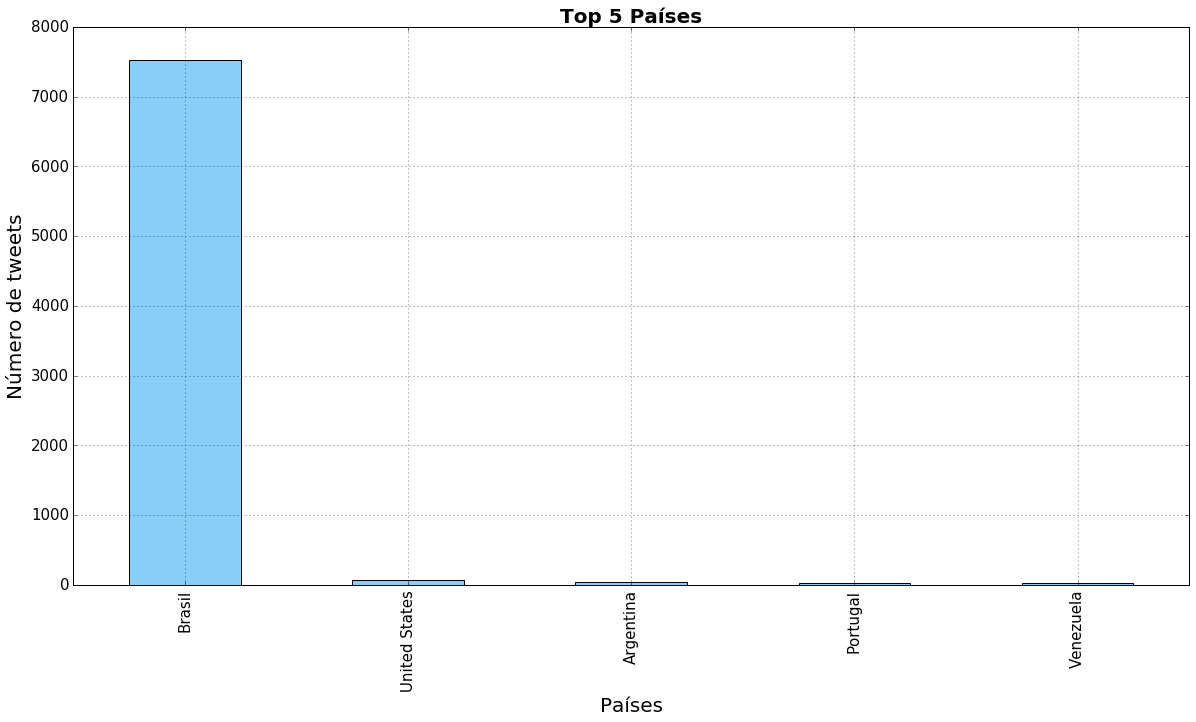
\includegraphics[width=1\textwidth]{Cap5/graficos/paises}}
	\caption{Países que mais realizaram \textit{tweets}}
	\vspace{-0.3cm}
	\legend{FONTE: Elaborado pelo autor}
	\label{paises}
\end{figure}

Este gráfico demonstra claramente que a maior número de \textit{tweets} foram publicados do Brasil e apenas uma pequena quantia deles foram realizados nos Estados Unidos, Argentina, Portugal e Venezuela. É importante notar que nem todos os \textit{tweets} gerados possuem um país de origem semelhante a situação anterior, onde a API do \textit{Twitter} os classificam como \textit{undefined}, porém não é apresentado no gráfico da Figura~\ref{paises}.

Utilizando uma biblioteca para expressões regulares, é possível procurar por \textit{tweets} de palavras específicas, ou \textit{hashtags} mesmo o usuário digitando com letras maiúsculas ou minúsculas.

O Código~\ref{cod-hash}, apresenta uma função que procura determinadas palavras dentro do \textit{DataFrame}. Estas palavras então preenchem uma coluna com os \textit{tweets} relacionados com a palavra buscada. As palavras buscadas são referentes às \textit{hashtags} que mais foram publicadas nesta data.

\lstinputlisting[language=Python, label=cod-hash, caption=Contabilização do número de \textit{tweets} por países]{Cap5/src/hashtags.py}

As \textit{hashtags} são contabilizadas e apresentadas através do gráfico de setores da Figura~\ref{hashtag}. Onde é possível verificar a porcentagem referente aos \textit{tweets} realizados com a \textit{hashtag} \#ImpeachmentDay. 

\begin{figure}[h]
	\centering
	\fbox{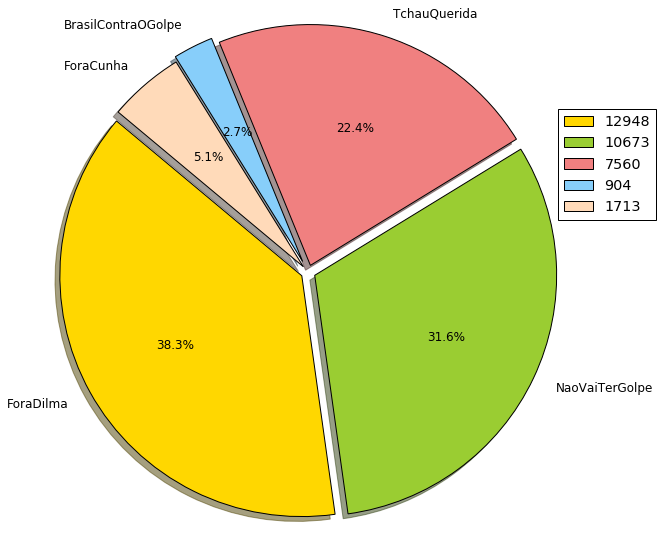
\includegraphics[width=1\textwidth]{Cap5/graficos/hashtag}}
	\caption{\textit{Hashtags} com o maior número de \textit{tweets}}
	\vspace{-0.3cm}
	\legend{FONTE: Elaborado pelo autor}
	\label{hashtag}
\end{figure}

Através da Figura~\ref{hashtag}, as \textit{hashtags} \#ForaDilma e \#TchauQuerida somam um total de 60,7\% que apoiam o processo de Impeachment  da presidente da República, diferente dos 34,3\% dos \textit{tweets} que é o somatório de \#BrasilContraOGolpe e \#NaoVaiTerGolpe.

Dando continuidade ao uso da biblioteca para trabalhar com expressões regulares, o Código~\ref{extract-link} permite encontrar \textit{links} que são publicados pelos usuários através de seus \textit{tweets}. Estes \textit{links} podem ser filtrados de acordo com a \textit{hashtag} utilizada.

\lstinputlisting[language=Python, label=extract-link, caption=Extração de \textit{links} provenientes de \textit{tweets}]{Cap5/src/extract-link.py}

O resultado da execução do Código~\ref{extract-link}, é uma lista de milhares de \textit{links} e o número em ordem do \textit{tweet} encontrado no \textit{DataFrame}. A Figura~\ref{links} apresenta um pedaço desta lista para exemplificação.

\begin{figure}[h]
	\centering
	\fbox{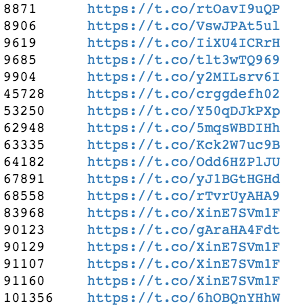
\includegraphics[width=0.5\textwidth]{Cap5/imagens/links}}
	\caption{Exemplo de \textit{links} extraídos de \textit{tweets}}
	\vspace{-0.3cm}
	\legend{FONTE: Elaborado pelo autor}
	\label{links}
\end{figure}

Semelhante ao Código~\ref{cod-hash}, é possível aplicar o filtro das \textit{hashtags} para encontrar nomes com maior popularidade através do Código~\ref{cod-fig-pol}.

\lstinputlisting[language=Python, label=cod-fig-pol, caption=Contabilização do número de \textit{tweets} por países]{Cap5/src/figuras-pol.py}

Como resultado o Código~\ref{cod-fig-pol}, constrói um gráfico de setores, nesse é possível verificar a porcentagem de \textit{tweets} para nomes específicos através da Figura~\ref{fig-pol}, porém não é possível, ainda, predizer se os argumentos a respeito destas pessoas são positivos ou negativos. \\ \\ \\ \\

\begin{figure}[h]
	\centering
	\fbox{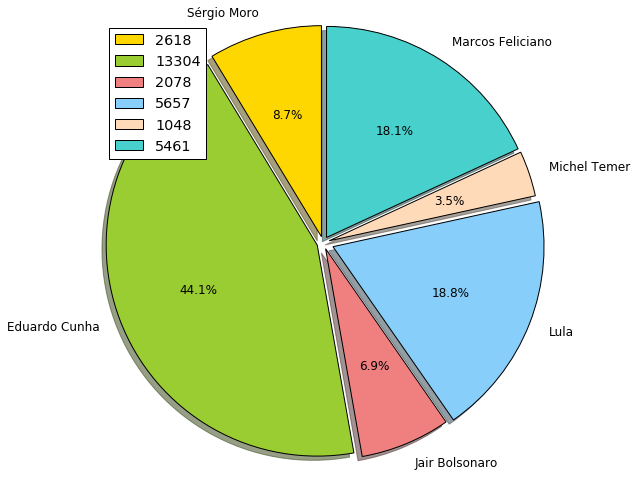
\includegraphics[width=1\textwidth]{Cap5/graficos/figuras-politicas}}
	\caption{Gráfico de setores para figuras importantes}
	\vspace{-0.3cm}
	\legend{FONTE: Elaborado pelo autor}
	\label{fig-pol}
\end{figure}

O gráfico de setores representado pela Figura~\ref{fig-pol}, demonstra que o nome mais mencionado foi de Eduardo Cunha e com apenas 2618 \textit{tweets} o nome de Michel Temer foi publicado. Até mesmo as menções ao ex-presidente Luiz Inácio "Lula" da Silva recebeu apenas 18,8\% do total dos nomes filtrados.































\chapter{ANÁLISE DOS RESULTADOS}\label{ch:conclusao}
% !TeX encoding = UTF-8

\chapter{CONCLUSÕES E SUGESTÕES PARA FUTUROS TRABALHOS}\label{ch:conclusao}
\section{CONCLUSÕES} 
O uso das bibliotecas que Python oferece para a mineração de dados...

- Resgatar o objetivo

- Comentar as ferramentas estudadas

- Comentar as ferramentas utilizadas

- Breve resumo dos resultados

- Pontos positivos e negativos (O fato de não ter o perfil real)


\section{SUGESTÕES PARA FUTUROS TRABALHOS}

%
%7.2
%Pensar em outra API (Aplicação para previsão de resultados) ou rede social, baseando-se numa pergunta específica

%\bookmarksetup{startatroot}

% ---
% ELEMENTOS PÓS-TEXTUAIS
% ---
\postextual

\bibliography{Configuracoes/citacoes} 		% Referências bibliográficas

% ---
% APÊNDICES
% ---

%\begin{apendicesenv}% Apêndices: inserir se necessário
%\partapendices
%  % ----------------------------------------------------------
\chapter{TENSORES} \label{Tensor}
% ----------------------------------------------------------

%\lipsum[50]

Na Física e nas Engenharias as grandezas podem ser classificadas em três grandes grupos:

\begin{enumerate}
	
	\item Grandezas escalares: são aquelas que necessitam de somente uma informação para classificá-las. Como exemplos destas grandezas tem-se a temperatura, comprimento, massa, tempo, volume, energia, entre outros.
	\item Grandezas vetoriais: são as que necessitam de três informações para caracterizá-las (módulo, direção e sentido). Como exemplos destas grandezas pode-se destacar o deslocamento, a força, o fluxo, a corrente elétrica e a aceleração.
	\item Grandezas Tensoriais: são aquelas que para serem bem representadas necessitam de, pelo menos, nove informações. Destacam-se como exemplos o tensor de tensão, o tensor de deformação, o tensor inercial e as rotações. 
\end{enumerate}

A transformação linear que tem a capacidade de transformar um dado vetor $ \vec{a} $ em um outro vetor $ \vec{b} $, ou seja,
\begin{equation}
	\vec{a} = \textbf{T} \vec{b}
\end{equation}
é chamada de tensor de segunda ordem ou simplesmente de tensor, cuja notação é $ \textbf{T} $. Assim, $ \textbf{T} $ é uma transformação linear, pois
\begin{equation}
	\textbf{T} ( \alpha \vec{a} + \beta \vec{b}) = \alpha \textbf{T}( \vec{a}) + \beta \textbf{T} ( \vec{b}).
\end{equation}

Para um conjunto de vetores unitários $ e_{1}, e_{2}, e_{3} $, na direção das componentes de um sistema de coordenadas retangulares, suas transformações podem ser escritas na forma
\begin{equation}
	\textbf{T} e_{1} = \textbf{T} \left[ 
	\begin{array}{c}
		1\\
		0\\
		0\\
	\end{array}
	\right] = \textbf{T} (1 e_{1} + 0 e_{2} + 0 e_{3}) 
\end{equation} 
ou
\begin{equation} \label{TFe1}
	\textbf{T} e_{1} = T_{11} e_{1} + T_{21} e_{2} + T_{31} e_{3},
\end{equation}
\begin{equation} \label{TFe2}
	\textbf{T} e_{2} = T_{12} e_{1} + T_{22} e_{2} + T_{32} e_{3},
\end{equation}
\begin{equation}\label{TFe3}
	\textbf{T} e_{3} = T_{13} e_{1} + T_{23} e_{2} + T_{33} e_{3}.
\end{equation}

Utilizando a notação indicial esta transformação pode ser generalizada como
\begin{equation} \label{indicialT}
	\textbf{T} e_{i} = T_{ji} e_{j}.
\end{equation}

Considerando as transformações apresentadas em (\ref{TFe1}), (\ref{TFe2}) e (\ref{TFe3}), o tensor \textbf{T} pode ser representado matricialmente da seguinte forma
\begin{equation} \label{matrizT}
	\textbf{T} = [T] =  \left[ 
	\begin{array}{ccc}
		T_{11} & T_{12} & T_{13} \\
		T_{21} & T_{22} & T_{23} \\
		T_{31} & T_{32} & T_{33} \\
	\end{array}
	\right].  
\end{equation} 

Assim como na transformação linear, os tensores também apresentam algumas propriedades. São elas:
\begin{enumerate}
	\item[a)] A soma entre dois tensores \textbf{T} e \textbf{S}
	\begin{equation}
		( \textbf{T} + \textbf{S}) \vec{a} = \textbf{T} \vec{a} + \textbf{S} \vec{a}, 
	\end{equation}
	que, em notação indicial, é escrito como
	\begin{equation}
		W_{ij} = T_{ij} + S_{ij}.
	\end{equation}
	\item[b)] O produto de dois tensores, caracteriza-se por
	\begin{equation}
		( \textbf{T} \textbf{S}) \vec{a} = \textbf{T} ( \textbf{S} \vec{a})
	\end{equation}
	ou
	\begin{equation}
		(TS)_{ij} = T_{im} S_{mj}.
	\end{equation}
	\item[c)] Transposição de um tensor $( \textbf{T} ^{T})$
	\begin{equation}
		\vec{a} \cdot \textbf{T} \vec{b} = \vec{b} \cdot \textbf{T} ^{T} \vec{a}.
	\end{equation}
	\item[d)] O traço de um tensor \textbf{T} é representado em notação indicial por
	\begin{equation}
		tr \textbf{T} = T_{ij} \delta _{ij},
	\end{equation}
	onde
	\begin{equation}
		\delta _{ij} = \left\{
		\begin{array}{rcl}
			1 & se & i = j\\
			0 & se & i \neq j
		\end{array} \right.,
	\end{equation}
	é o delta de Kronecker.
	\item[e)] Um tensor \textbf{T} pode ser decomposto em uma parte simétrica, $ \textbf{T} ^{S} $, e uma parte antissimétrica, $ \textbf{T} ^{A} $, ou seja,
	\begin{equation}
		\textbf{T} = \textbf{T} ^{S} + \textbf{T} ^{A},
	\end{equation}
	\begin{equation}
		\textbf{T} ^{S} = \dfrac{ \textbf{T} + \textbf{T} ^{T}}{2},
	\end{equation}
	e
	\begin{equation}
		\textbf{T} ^{A} = \dfrac{ \textbf{T} - \textbf{T} ^{T}}{2}.
	\end{equation}
\end{enumerate}

No cálculo tensorial, se $ \textbf{T} = \textbf{T} (t) $ for um tensor de segunda ordem dependente do tempo, então
\begin{equation}
	\dfrac{d \textbf{T}}{dt} = \lim_{ \Delta t \to 0} \dfrac{ \textbf{T} ( t+ \Delta t) - \textbf{T} (t)}{ \Delta (t)}
\end{equation}
e
\begin{equation}
	\dfrac{d}{dt} [ \textbf{T} + \textbf{S}] = \dfrac{d \textbf{T}}{dt} + \dfrac{d \textbf{S}}{dt}.
\end{equation}

Se $ \alpha(t)$ for um escalar dependente do tempo, então
\begin{equation}
	\dfrac{d}{dt}  [ \alpha(t) \textbf{T}] = \dfrac{d \alpha(t)}{dt} \textbf{T} + \alpha(t) \dfrac{d \textbf{T}}{dt}.
\end{equation}

Se $ [ \textbf{T} \textbf{S}]$ for o produto entre dois tensores, então
\begin{equation}
	\dfrac{d}{dt} [ \textbf{T} \textbf{S}] = \dfrac{d \textbf{T}}{dt} \textbf{S} + \textbf{T} \dfrac{d \textbf{S}}{dt}. 
\end{equation}

Se $ [ \textbf{T} \vec{a}]$ representa a transformação de um vetor $ \vec{a}$, então
\begin{equation}
	\dfrac{d}{dt} [ \textbf{T} \vec{a}] = \dfrac{d \textbf{T}}{dt} \vec{a} + \textbf{T} \dfrac{d \vec{a}}{dt}.
\end{equation}

Se $[ \textbf{T} ^{T}]$ representar um tensor transposto, então
\begin{equation}
	\dfrac{d}{dt} [ \textbf{T} ^{T}] =
	\left[
	\begin{array}{c}
		\dfrac{d \textbf{T}}{dt}\\
	\end{array} \right] ^{T} .
\end{equation}

Para um campo vetorial o divergente de um vetor velocidade $ \vec{v}$ é calculado, segundo \citeonline{Malvern}, por
\begin{equation}
	\mbox{div} \vec{v} = tr [ { \nabla} \vec{v}] = { \nabla} \cdot \vec{v}
\end{equation} 
onde $ { \nabla} $ é o operador gradiente. Assim, tem-se que, em relação às suas componentes,
\begin{equation}
	\mbox{div} \vec{v} = \dfrac{ \partial v_{1}}{ \partial x_{1}} + \dfrac{ \partial v_{2}}{ \partial x_{2}} +\dfrac{ \partial v_{3}}{ \partial x_{3}}.
\end{equation}

Para um campo tensorial, o divergente deste campo é calculado pela equação
\begin{equation}
	(\mbox{div} \textbf{T}) \cdot \vec{a} = \mbox{div} ( \textbf{T} ^{T} \vec{a}) - tr ( \textbf{T} ^{T} ( { \nabla} \vec{a}))
\end{equation}
ou, em notação indicial,
\begin{equation}
	\mbox{div} \textbf{T} = \dfrac{ \partial T_{im}}{ \partial x_{m}} \vec{e} _{i}.
\end{equation}

Em certos problemas da engenharia que envolvem pequenos deslocamentos faz-se necessário conhecer e descrever suas deformações. Quando estas deformações são muito pequenas dá-se o nome de deformações infinitesimais \cite{Lai}.

Considerando a Figura \ref{fig:campodeform}, em um dado instante $ t_{0} $, os pontos $ P(t_{0}) $ e $ Q(t_{0}) $ apresentam um vetor distância $ \vec{dX} $. Para este instante $ t_{0} $ diz-se que os pontos estão na configuração $ B_{0} $. Após um certo instante de tempo $ t $ ocorre o deslocamento dos pontos $ P $ e $ Q $, sendo chamados agora de $ P(t) $, $ Q(t) $  e a nova configuração de $ B_{t} $, o que infere uma mudança em $  \vec{dX} $ passando a ser chamado de $  \vec{dx} $. Esta variação de deslocamento, por ser infinitesimal, pode ser considerada como um filamento. Logo, o filamento  $  \vec{dx} $ é dado por:
\begin{equation} \label{filamento}
	\vec{dx} = \vec{dX} + ( { \nabla} \vec{u}) \vec{dX},
\end{equation}
onde
\begin{equation}
	{ \nabla} \vec{u} = \left[
	\begin{array}{ccc}
		\dfrac{ \partial u_{1}}{ \partial x_{1}} & \dfrac{ \partial u_{1}}{ \partial x_{2}} & \dfrac{ \partial u_{1}}{ \partial x_{3}}\\
		
		\dfrac{ \partial u_{2}}{ \partial x_{1}} & \dfrac{ \partial u_{2}}{ \partial x_{2}} & \dfrac{ \partial u_{3}}{ \partial x_{3}}\\
		
		\dfrac{ \partial u_{3}}{ \partial x_{1}} & \dfrac{ \partial u_{3}}{ \partial x_{2}} & \dfrac{ \partial u_{3}}{ \partial x_{3}}\
	\end{array} \right],
\end{equation}
é o tensor gradiente de deslocamentos.

\begin{figure}[H]
	\centering
	\includegraphics[scale=1]{figuras/campo_de_deformacao.jpg}
	\caption{\textsc{Deformação infinitesimal}}
	\vspace{-0.1cm}
	\legend{FONTE: \citeonline{Lai}}
	\label{fig:campodeform}
\end{figure}

%\begin{figure}
%\caption{DEFORMAÇÃO INFINITESIMAL}
%\small{Fonte: LAI, 2010}
%\label{fig:campodeform}
%\centering
%\includegraphics[scale=1]{campo_de_deformacao.jpg}
%\end{figure}	


O filamento $ \vec{dx} $ na equação (\ref{filamento}) pode ser escrita como 
\begin{equation}
	\vec{dx} = [ \textbf{I} + ( { \nabla} \vec{u})] \vec{dX} 
\end{equation}
onde \textbf{I} é o  tensor identidade. Logo, 
\begin{equation} \label{filamento_dx}
	\vec{dx} = \textbf{F} \vec{dX},
\end{equation}
sendo
\begin{equation} \label{tensordeform}
	\textbf{F} = \textbf{I} + ( { \nabla}  \vec{u}).
\end{equation}
Mas
\begin{equation}
	\textbf{F} ^T \cdot \textbf{F} = ( \textbf{I} + { \nabla}  \vec{u}) ^T \cdot ( \textbf{I} + { \nabla}  \vec{u}) 
\end{equation}
o que resulta em
\begin{equation} \label{FtranspF}
	\textbf{F} ^T \cdot \textbf{F} = \textbf{I} + ( { \nabla}  \vec{u}) + ( { \nabla}  \vec{u}) ^T +  ( { \nabla}  \vec{u}) ^T ( { \nabla}  \vec{u}).
\end{equation}

Considerando que a magnitude do vetor $  \vec{u} $ é muito pequena, $  \Vert \vec{u} \Vert < < 1  $ , então       
\begin{equation}
	( { \nabla}  \vec{u}) ^T ( { \nabla}  \vec{u}) \approx 0,
\end{equation}
que, substituindo na equação (\ref{FtranspF}), resulta
\begin{equation}
	\textbf{F} ^T \cdot \textbf{F} = \textbf{I} + ( { \nabla}  \vec{u}) + ( { \nabla}  \vec{u}) ^T .
\end{equation}

Assumindo
\begin{equation}
	\textbf{E} = \dfrac{ ( { \nabla}  \vec{u}) + ( { \nabla}  \vec{u}) ^T}{2}
\end{equation}
como sendo um tensor simétrico de $ ( { \nabla}  \vec{u})   $, então
\begin{equation}
	\textbf{F} ^T \cdot \textbf{F} = \textbf{I} + 2 \textbf{E},
\end{equation}      
sendo \textbf{E} chamado de tensor de deformações infinitesimais.
Assim com foi feito nas equações (\ref{indicialT}) e (\ref{matrizT}), o tensor \textbf{E} também pode ser escrito na forma matricial
\begin{equation}
	[E] =  \left[ 
	\begin{array}{ccc}
		E_{11} & E_{12} & E_{13} \\
		E_{21} & E_{22} & E_{23} \\
		E_{31} & E_{32} & E_{33} \\
	\end{array}
	\right] _{X_{1} X_{2} X_{3}}.  
\end{equation}

No entanto, se as deformações ocorrerem somente nas direções principais, ou seja, nas direções dos autovetores  do tensor \textbf{E}, então
\begin{equation}
	[E] =  \left[ 
	\begin{array}{ccc}
		E_{1} & 0 & 0 \\
		0 & E_{2} & 0 \\
		0 & 0 & E_{3} \\
	\end{array}
	\right]  
\end{equation}
e, neste caso, haverá na transformação uma preservação dos ângulos, sendo chamada de uma transformação pura \cite{Lai}.

\begin{figure}[H]
	\centering
	\includegraphics[scale=1]{figuras/deformacoes.jpg}
	\caption{\textsc{Campo de deslocamentos}}
	\vspace{-0.1cm}
	\legend{FONTE: \citeonline{Lai}}
	\label{fig:campodesl}
\end{figure}

%\begin{figure}
%\caption{CAMPO DE DESLOCAMENTOS}
%\label{fig:campodesl}
%\centering
%\includegraphics[scale=1]{deformacoes.jpg}
%\end{figure}


A Figura \ref{fig:campodesl} apresenta o deslocamento de um dado corpo rígido no instante $ t_{0} $ e após um instante $ t $. Nota-se, em relação à sua configuração inicial, que este corpo sofreu dois movimentos, sendo um de rotação e o outro de deformação. Assim, sejam \textbf{U} e \textbf{V} tensores simétricos e \textbf{R} um tensor ortogonal próprio. Tomando como base a equação (\ref{tensordeform}), o tensor \textbf{F} pode ser escrito como
\begin{equation} \label{Caucy_dir}
	\textbf{F} = \textbf{R} \textbf{U}
\end{equation}    
e
\begin{equation} \label{Caucy_esq}
	\textbf{F} = \textbf{V} \textbf{R}.
\end{equation}


%-----------------------------------------------------
%para trabalhar com referencias para equações
%incluir o label com um nome para a equacao e referenciar no texto com ~\ref{label} 
%\begin{equation}\label{nome}
%\textbf{F} = \textbf{V} \textbf{R}.
%\end{equation}
%-----------------------------------------------------

As equações (\ref{Caucy_dir}) e (\ref{Caucy_esq}) são conhecidas como Teorema de decomposição polar e os tensores \textbf{U} e \textbf{V} como tensores de \textit{Strech} à direita e à esquerda, respectivamente.

Utilizando as equações (\ref{Caucy_dir}) e (\ref{Caucy_esq}), a equação (\ref{filamento_dx}) pode ser escrita da seguinte forma
\begin{equation}
	\vec{dx} =  \textbf{F} \vec{dX} = \textbf{R} \textbf{U} \vec{dX} = \textbf{R} ( \textbf{U} \vec{dX}),
\end{equation}
onde pode-se afirmar que, inicialmente, o corpo está sofrendo uma deformação pura (\textit{Strech}) e, após, uma rotação. Mas, pela equação (\ref{Caucy_esq}), pode-se ter também que
\begin{equation}
	\vec{dx} =  \textbf{F} \vec{dX} = \textbf{V} \textbf{R} \vec{dX} = \textbf{V} ( \textbf{R} \vec{dX}),
\end{equation}
onde inicialmente o corpo sofre uma rotação e então uma deformação. Em ambos os casos, o resultado será sempre o mesmo, como pode ser observado na Figura \ref{fig:campodeform}.

Dos tensores \textbf{U} e \textbf{V} surgem conceitos de significativa importância nas engenharias. Para tanto, seja
\begin{equation}
	\textbf{C} = \textbf{U} ^{2},
\end{equation}
onde o tensor \textbf{C} é chamado de tensor deformação de Cauchy-Green à direita, pois na equação (\ref{Caucy_dir}) o tensor \textbf{U} encontra-se à direita. Como este tensor é simétrico e o tensor \textbf{R} é ortogonal, tem-se
\begin{equation} \label{CG_direita}
	\textbf{C} = \textbf{F} ^{T} \textbf{F}.
\end{equation}

As componentes do tensor de Cauchy-Green à direita, $ C_{ij} $, tomando como base o tensor \textbf{F}, representam uma razão quadrática da medida  de deformação entre dois filamentos $ \vec{dx} ^{ (1)} $ e $ \vec{dx} ^{ (2)} $, se $ i=j $. Caso $ i \neq j $, $ C_{ij} $ irá representar a medida de distorção angular entre os dois filamentos.

Se as deformação não forem mais infinitesimais, mas sim finitas, tem-se o tensor Lagrangeano de deformações, $ \textbf{E} ^{*}$, sendo
\begin{equation}
	\textbf{E} ^{*} = \dfrac{1}{2} [( { \nabla} \vec{u}) + ( { \nabla} \vec{u}) ^{T}] + \dfrac{1}{2} ( { \nabla} \vec{u}) ^{T} ( { \nabla} \vec{u})
\end{equation}  
ou
\begin{equation}
	\textbf{E} ^{*} = \dfrac{1}{2} ( \textbf{C} - \textbf{I}).
\end{equation}

Em notação indicial o tensor Lagrangeano de deformações é escrito como
\begin{equation}
	E_{ij} ^{*} = \dfrac{1}{2} \left[ \dfrac{ \partial u_{i}}{ \partial X_{j}} + \dfrac{ \partial u_{j}}{ \partial X_{i}} \right] + \dfrac{1}{2} \dfrac{ \partial u_{m}}{ \partial X_{i}}  \dfrac{ \partial u_{m}}{ \partial X_{j}},
\end{equation}
onde $m$ e $n$ resultam de vetores unitários não mutuamente perpendiculares.

Seja \begin{equation}
	\textbf{B} = \textbf{V} ^{2},
\end{equation}
então o tensor \textbf{B} é chamado de tensor de Cauchy-Green à esquerda, pois na equação (\ref{Caucy_esq}) o tensor \textbf{V} está à esquerda. 

Assim como na equação (\ref{CG_direita}), tem-se 
\begin{equation}
	\textbf{B} = \textbf{V} ^{2} = \textbf{F} \textbf{F} ^{T} = ( \textbf{I} + { \nabla} \vec{u}) ( \textbf{I} + { \nabla} \vec{u}) ^{T}.
\end{equation}
Logo,
\begin{equation}
	\textbf{B} = \textbf{I} + [ { \nabla} \vec{u} + ( { \nabla} \vec{u}) ^{T}] + ( { \nabla} \vec{u}) ( { \nabla} \vec{u}) ^{T}
\end{equation}
que, em notação indicial, torna-se
\begin{equation} \label{comp_CG_esquerda}
	B_{ij} = \delta _{ij} + \left[ \dfrac{ \partial u_{i}}{ \partial X_{j}} + \dfrac{ \partial u_{j}}{ \partial X_{i}} \right] +  \dfrac{ \partial u_{i}}{ \partial X_{m}}  \dfrac{ \partial u_{j}}{ \partial X_{m}}.
\end{equation}

Se na equação (\ref{comp_CG_esquerda}) $ i=j $, assim como ocorre no tensor de Cauchy-Green à direta, $ B_{ij} $ representará a razão quadrática da medida de deformação entre os filamentos $ \vec{dx} ^{ (1)} $ e  $ \vec{dx} ^{ (2)} $. Caso $ i \neq j $, $ B_{ij} $ representará o quanto o ângulo entre os filamentos deixa de ser reto.

Se as deformações não forem mais infinitesimais, mas sim finitas, tem-se o tensor Euleriano de deformações,  $ \textbf{e} ^{*}$, sendo  
\begin{equation}
	\textbf{e} ^{*} = \dfrac{1}{2} [( { \nabla} \vec{u}) + ( { \nabla} \vec{u}) ^{T}] - \dfrac{1}{2} ( { \nabla} \vec{u}) ^{T} ( { \nabla} \vec{u})
\end{equation}
ou
\begin{equation}
	\textbf{e} ^{*} = \dfrac{1}{2} ( \textbf{I} - \textbf{B} ^{-1}).
\end{equation}

Em notação indicial o vetor $ \textbf{e} ^{*}$ torna-se
\begin{equation}
	e_{ij} ^{*} = \dfrac{1}{2} \left[ \dfrac{ \partial u_{i}}{ \partial X_{j}} + \dfrac{ \partial u_{j}}{ \partial X_{i}} \right] - \dfrac{1}{2} \dfrac{ \partial u_{m}}{ \partial X_{i}}  \dfrac{ \partial u_{m}}{ \partial X_{j}}.
\end{equation}

Um dado corpo é dito em equilíbrio se a resultante das forças que atuam sobre ele é nula \cite{Malvern}. Em outras palavras,
\begin{equation}
	\sum \vec{F} = 0.
\end{equation}  

Seja $ S $ um plano que passa em algum ponto arbitrário $ P $ de um corpo que possui $  \vec{n} $ como seu vetor normal unitário. Ao ser aplicada uma força externa  $ \vec{F}$ neste corpo o ponto $ P $ sofrerá uma tensão (pressão) que é dada pela razão da decomposição da força $ \vec{F} $, em relação à normal $ \vec{n} $, pela variação de área. A medida que a área diminui atingi-se um valor limite da tensão, 
\begin{equation}
	\vec{t} = \lim_{ A_{S} \to 0} \dfrac{ \Delta \vec{F}}{ \Delta A_{S}}
\end{equation}  
onde $ \vec{t} $ é chamado de vetor tensão e é entendido como a força resultante no ponto $ P $ em uma área infinitesimal. Por esta característica, o vetor tensão $ \vec{t} $ tem dimensão de pressão, isto é, $ N/m^{2} $, $ kgf/cm^{2} $, $ lb/in^{2} $ \cite{Lai}.

\begin{figure}[H]%COLOCAR FIGURA PAG 155 LAI
	\centering
	\includegraphics[scale=1]{figuras/vetor_tensao.jpg}
	\caption{\textsc{Plano de formação do vetor de tensão}}
	\vspace{-0.1cm}
	\legend{FONTE: \citeonline{Lai}}
	\label{fig:vetortensao}
\end{figure}
%\begin{figure}%COLOCAR FIGURA PAG 155 LAI
%\caption{PLANO DE FORMAÇÃO DO VETOR DE TENSÃO}
%\label{fig:vetortensao}
%\centering
%\includegraphics[scale=1]{vetor_tensao.jpg}
%\end{figure}	

O vetor tensão $  \vec{t} $ depende tanto da posição do ponto $ P $ como também da normal do plano $ S $. Assim,
\begin{equation}
	\vec{t} = \vec{t} ( \vec{x}, t, \vec{n}) = \textbf{T} ( \vec{x}, t) \vec{n}
\end{equation} 
ou, simplesmente,
\begin{equation} \label{vetor_tensao}
	\vec{t} _{ \vec{n}} = \textbf{T} \vec{n}.
\end{equation}

\begin{figure}[H]%COLOCAR A FIGURA 4.2.1 PAG 157
	\centering
	\includegraphics[scale=1]{figuras/componentes_vetor_tensao.jpg}
	\caption{\textsc{Componentes do vetor de tensão}}
	\vspace{-0.1cm}
	\legend{FONTE: \citeonline{Lai}}
	\label{fig:compvetortensao}
\end{figure}
%\begin{figure}%COLOCAR A FIGURA 4.2.1 PAG 157
%\caption{COMPONENTES DO VETOR DE TENSÃO}
%\label{fig:compvetortensao}
%\centering
%\includegraphics[scale=1]{componentes_vetor_tensao.jpg}
%\end{figure}	

Tomando como base a Figura \ref{fig:compvetortensao} o vetor de tensões pode ser escrito em função das suas componentes como
\begin{equation}
	\vec{t} _{ \vec{n}} = n_{1} \vec{t} _{ \vec{e} _{1}} + n_{2} \vec{t} _{ \vec{e} _{2}} + n_{3} \vec{t} _{ \vec{e} _{3}}.
\end{equation}

Assim,
\begin{equation} \label{componente_vetor_tensao}
	\begin{array}{c}
		\vec{t} _{ \vec{e} _{1}} = T_{11} \vec{e} _{1} + T_{21} \vec{e} _{2} + T_{31} \vec{e} _{3}\\
		\vec{t} _{ \vec{e} _{2}} = T_{21} \vec{e} _{1} + T_{22} \vec{e} _{2} + T_{32} \vec{e} _{3}\\
		\vec{t} _{ \vec{e} _{3}} = T_{31} \vec{e} _{1} + T_{31} \vec{e} _{2} + T_{33} \vec{e} _{3}\\
	\end{array}
\end{equation}
ou, utilizando notação indicial,
\begin{equation}
	\vec{t} _{ \vec{e} _{i}} = T_{mi} \vec{e} _{m},
\end{equation}
sendo $ T_{mi} $ com $ m=i  $, chamado componente tangencial, $ \sigma _{ \vec{n}} $, e quando $ m \neq i  $, $ T_{mi} $ é chamado de componente cisalhante, $ \vec{\tau} _{S}$, cuja magnitude é calculada por
\begin{equation}
	\Vert \vec{\tau} _{S} \Vert = \sqrt{ \Vert \vec{t} _{ \vec{n}} \Vert ^{2} - \Vert \sigma _{ \vec{n}} \Vert ^{2}}.
\end{equation}

De acordo com as equações (\ref{vetor_tensao}) e (\ref{componente_vetor_tensao}), $ \textbf{T} $ é uma transformação linear sendo chamado de tensor de tensões ou tensor de tensões de Cauchy \cite{Lai}.

O tensor de tensões de Cauchy, de acordo com a sua formulação, está definido na configuração deformada $ B_{t} $, conforme pode ser observado nas Figuras \ref{fig:campodesl} e \ref{fig:campodeform}. No entanto, em certos problemas das engenharias, há a necessidade de se avaliar os estados de tensões na configuração $ B_{0} $. Para tanto, seja $ \vec{df} $ um vetor força definido em uma área infinitesimal $ dA $. Então, 
\begin{equation}
	\vec{df}  = \vec{t} dA
\end{equation}
onde, pela equação (\ref{vetor_tensao}), 
\begin{equation}
	\vec{t} = \textbf{T} \vec{n}.
\end{equation}

Se for possível escrever o vetor $ \vec{df} $ em função de um vetor tensão, $ \vec{t} _{0} $, em $ B_{0} $ e em relação a uma área indeformada, então
\begin{equation}
	\vec{df}  = \vec{t} dA \Longleftrightarrow \vec{df}  = \vec{t_{0}} dA_{0}.
\end{equation}
Logo,
\begin{equation}
	\vec{df}  = \vec{t} dA  = \vec{t_{0}} dA_{0},
\end{equation}
isto é,
\begin{equation}
	\vec{t_{0}} = \dfrac{dA}{dA_{0}} \vec{t}
\end{equation}
que, pela equação (\ref{vetor_tensao}),
\begin{equation} \label{vetor_tensao_B0}
	\vec{t}_{0} = \textbf{T}_{0} \vec{n}_{0} = \textbf{T} \dfrac{dA}{dA_{0}} \vec{n}. 
\end{equation}

Como, segundo \citeonline{Malvern}, 
\begin{equation}
	dA \vec{n} = dA_{0} \vert \textbf{F} \vert ( \textbf{F} ^{-1}) ^{T} \vec{n} _{0}
\end{equation}
a equação em (\ref{vetor_tensao_B0}) pode ser escrita como
\begin{equation}
	\vec{t}_{0}  \vec{n} _{0} = \textbf{T}  \vert \textbf{F} \vert ( \textbf{F} ^{-1}) ^{T} \vec{n} _{0}.
\end{equation}
Logo,
\begin{equation} \label{tensor_PK}
	\textbf{T} _{ \textbf{0}} = \textbf{T}  \vert \textbf{F} \vert ( \textbf{F} ^{-1}) ^{T},
\end{equation}
onde $ \textbf{T} _{ \textbf{0}} $ é conhecido como o primeiro tensor de Piolla-Kirchhoff.

Como o tensor de tensões de Cauchy \textbf{T} é simétrico e o tensor \textbf{F} não é simétrico, o primeiro tensor de Piolla-Kirchhoff não será simétrico. Para contornar tal problema pode-se considerar um  "pseudo" \ tensor força $ \tilde{df} $ na área $ dA_{0} $, onde
\begin{equation}
	\tilde{df} = \tilde{t} dA_{0}
\end{equation} 
sendo $ \tilde{t} $ um "pseudo" \ vetor tensão na área $ dA_{0} $, calculado por
\begin{equation}
	\tilde{t} =  \tilde{ \textbf{ T}} \vec{n} _{0}.
\end{equation}

Procedendo de forma análoga ao que foi feito com primeiro tensor de Piolla-Kirchhoff, obtêm-se
\begin{equation}
	\tilde{ \textbf{ T}}  = \textbf{F} ^{-1} \textbf{T} _{0}
\end{equation}
ou, pela equação (\ref{tensor_PK}),
\begin{equation}
	\tilde{ \textbf{T}} = \vert \textbf{F} \vert ( \textbf{F} ^{-1}) \textbf{T}   ( \textbf{F} ^{-1}) ^{T},
\end{equation}
sendo agora $ \tilde{ \textbf{T}} $ simétrico e chamado de segundo tensor de Piolla-Kirchhoff.




%  % ----------------------------------------------------------
\chapter{MODELO HÍBRIDO}

Modelo híbrido desenvolvido, em Pascal, para solucionar o problema da ruptura de barragens governado pelas equações de Águas Rasas unidimensional. 

\begin{verbatim}

	program rb02;
	
	uses
	wincrt;
	
	type
	vet = array[0..1000] of double;
	
	var
	az,au   : text;
	x       : ^vet;
	u,z     : array[1..2] of ^vet;
	t,ti,
	c0,zm,
	dx,dt,
	msdx,z0 : double;
	i,i2,
	nx1,
	nx2     : integer;
	
	const
	h  : double  = 1.0;
	lp : double  = 2.0;
	lg : double  = 4.0;
	g  : double  = 9.807;
	ep : double  = 0.00001;
	nx : integer = 400;
	ni : integer = 500;
	
	
	procedure sol_ex(t:double);
	
	var
	x1,x2,a : double;
	i1,i2,i : integer;
	
	begin
	
	x1 := h - t*c0;
	x2 := h + 2.0*t*c0;
	
	i1 := trunc(ep+(x1/dx));
	i2 := trunc(ep+(x2/dx));
	
	for i := i1+1 to i2-1 do
	begin
	
	a := (2.0*c0 + (h-x^[i])/t)/3.0;
	
	z[2]^[i] := a*a/g;
	u[2]^[i] := 2.0*(c0 - a);
	
	end;
	
	end;
	
	procedure sol_num(t:double);
	
	var
	dzdx,dudx,
	a,zx,ux,
	zmed      : double;
	i1,i2,i   : integer;
	
	begin
	
	z[1] := z[2];
	u[1] := u[2];
	
	for i := 1 to nx1 do
	begin
	
	i1 := i - 1;
	i2 := i + 1;
	
	zx := 0.5*(z[1]^[i1] + z[1]^[i2]);
	ux := 0.5*(u[1]^[i1] + u[1]^[i2]);
	
	dzdx := msdx*(z[1]^[i2] - z[1]^[i1]);
	dudx := msdx*(u[1]^[i2] - u[1]^[i1]);
	
	a := ux*dudx + g*dzdx;
	u[2]^[i] := ux - a*dt;
	
	a := zx*dudx + ux*dzdx;
	z[2]^[i] := zx - a*dt;
	
	end;
	
	z[2]^[0]  := z[2]^[1];
	z[2]^[nx] := z[2]^[nx-1];
	
	zmed := 0.0;
	for i := 0 to nx do
	zmed := zmed + z[2]^[i];
	
	a := nx*zm/zmed;
	for i := 0 to nx do
	z[2]^[i] := a*z[2]^[i];
	
	end;
	
	procedure gravar(t:double);
	
	var
	i : integer;
	
	begin
	
	writeln(az);
	write  (az,t);
	
	writeln(au);
	write  (au,t);
	
	i := 0;
	repeat
	
	write(az,' ',z[2]^[i]);
	write(au,' ',u[2]^[i]);
	
	i := i + nx2;
	
	until i > nx;
	(*
	write(az,' ',z[2]^[nx]);
	write(au,' ',u[2]^[nx]);
	*)
	end;
	
	begin
	
	new(x);
	for i := 1 to 2 do
	begin
	new(u[i]);
	new(z[i]);
	end;
	
	nx1  := nx - 1;
	nx2  := nx div 20;
	dx   := lg/nx;
	dt   := 0.01*dx;
	msdx := 0.5/dx;
	
	i2 := trunc((h/dx)+ep);
	
	for i := 0 to nx do
	begin
	x^[i]    := i*dx;
	u[2]^[i] := 0.0;
	end;
	
	for i := 0 to i2 do
	z[2]^[i] := lp;
	
	for i := i2+1 to nx do
	z[2]^[i] := 0.0;
	
	zm := lp*h/lg;
	c0 := sqrt(g*lp);
	
	writeln(zm);
	
	t  := h/c0;
	ti := 0.5*(lg-h)/c0;
	
	if ti > t
	then
	ti := t;
	
	writeln(ti);
	readln;
	
	assign(az,'rb02z.txt');
	assign(au,'rb02u.txt');
	
	rewrite(az);
	rewrite(au);
	
	writeln(az);
	write  (az,'        t(s)\x(m)      ');
	writeln(au);
	write  (au,'        t(s)\x(m)      ');
	
	i := 0;
	repeat
	
	write(az,' ',x^[i]);
	write(au,' ',x^[i]);
	
	i := i + nx2;
	
	until i > nx;
	(*
	write(az,' ',x^[nx]);
	write(au,' ',x^[nx]);
	*)
	t := ni*dt;
	repeat
	
	writeln(t);
	
	sol_ex(t);
	
	writeln(t,z[2]^[0],z[2]^[nx]);
	
	gravar(t);
	
	t := t + ni*dt;
	
	until t > ti;
	
	t := t - ni*dt;
	
	repeat
	
	z0 := z[2]^[0];
	
	for i := 1 to ni do
	begin
	
	t := t + dt;
	
	sol_num(t);
	
	end;
	
	gravar(t);
	
	writeln(t,z[2]^[0],z[2]^[nx]);
	
	until abs(z0-z[2]^[0]) < ep;
	
	close(az);
	close(au);
	
	end.
	
\end{verbatim}

% ----------------------------------------------------------
%\lipsum[55-57]
%\end{apendicesenv}

%\begin{anexosenv}% Anexos: inserir se necessário
%\partanexos
% % ---
\chapter{Morbi ultrices rutrum lorem.}
% ---
\lipsum[30]


% % ---
\chapter{Cras non urna sed feugiat cum sociis natoque penatibus et magnis dis
parturient montes nascetur ridiculus mus}
% ---

\lipsum[31]

% 
% ---
\chapter{Fusce facilisis lacinia dui}
% ---

\lipsum[32]

%\end{anexosenv}

\printindex		% Indice Remissivo
\end{document}
